\RequirePackage{fix-cm} % Added by the template.

% smallextended below is the one used by MPC,  see:
% https://www.springer.com/journal/12532/submission-guidelines
\documentclass[smallextended]{svjour3}       % onecolumn (second format)

% FIX cleverref + svjour3 bug, see:
% https://tex.stackexchange.com/questions/499497/
\makeatletter
\let\cl@chapter\undefined
\makeatletter

\smartqed  % flush right qed marks, e.g. at end of proof

% insert here the call for the packages your document requires
\usepackage{mathptmx} % use the same font the Journal will use if possible
% packages for diagrams and colored links
\usepackage{graphicx} % already present in template, do not remove
\usepackage{multirow}
% The hypertexnames is necessary to remove a lot of warnings about
% figure and table repeated names. It seems the template does something
% wrong with the kind of counter used to mark these places.
\usepackage[hypertexnames=false]{hyperref}
\usepackage{color}
\usepackage[table]{xcolor}
\definecolor{gray-table-row}{gray}{0.90}
% Packages for computer code
\usepackage{algorithm}
\usepackage{algpseudocode}
% Package for multiline comments
\usepackage{verbatim}
% Packages for formatting the mathematical formulation
\usepackage{mathtools}
\usepackage{amsmath}
\usepackage{amssymb}
\usepackage[nameinlink]{cleveref}
\usepackage[normalem]{ulem} % for \sout
\usepackage{tikz}

% To differ between the text before the major revision and after it.
\newif\iffinalversion
%\finalversiontrue
\newcommand{\newtext}[1]{\iffinalversion%
#1%
\else%
\textcolor{blue}{#1}%
\fi%
}
\newcommand{\oldtext}[1]{\iffinalversion%
\else%
\textcolor{red}{#1}%
\fi%
}
\finalversiontrue

% please place your own definitions here and don't use \def but \newcommand
\newcommand{\isep}{\mathrel{{.}\,{.}}\nobreak} % for integer ranges
% sorry, but def needs to be used in this case
\def\sectionautorefname{Section} % change hyperref autoref to capitalized
\def\subsectionautorefname{Section} % change hyperref autoref to capitalized
\def\subsubsectionautorefname{Section} % change hyperref autoref to capitalized
\newcommand{\orcid}[1]{\href{https://orcid.org/#1}{[#1]}}

% Insert the name of "your journal" with
\journalname{Mathematical Programming Computation}

\begin{document}

\title{Enhanced Formulation for \newtext{the} Guillotine 2D Cutting \newtext{Knapsack} Problem\oldtext{s}}
%\subtitle{Do you have a subtitle?\\ If so, write it here}

%\titlerunning{Short form of title}        % if too long for running head

\author{Henrique Becker\orcid{0000-0003-3879-2691} \and Olinto Araujo\orcid{0000-0003-1136-5032} \and Luciana S. Buriol\orcid{0000-0002-9598-5732}}
%\author{Henrique Becker \and Olinto Araujo \and Luciana S. Buriol}

\authorrunning{H. Becker et al.} % if too long for running head

\institute{
	Henrique Becker \at
	Federal University of Rio Grande do Sul (UFRGS), Av. Bento Gonçalves, 9500, Porto Alegre, RS, Brazil\\
	% Postgraduate on Computer Science Program
	%Tel.: +123-45-678910\\
	%Fax: +123-45-678910\\
	\email{hbecker@inf.ufrgs.br}           %  \\
	%\emph{Present address:} of F. Author  %  if needed
\and
	Olinto Araujo \at
	Federal University of Santa Maria (UFSM), Av. Roraima, 1000, Santa Maria, RS, Brazil\\
	% Postgraduate on Production Engineering Program
	%Tel.: +123-45-678910\\
	%Fax: +123-45-678910\\
	\email{olinto@ctism.ufsm.br}           %  \\
	%\emph{Present address:} of F. Author  %  if needed
\and
	Luciana S. Buriol \at
	Federal University of Rio Grande do Sul (UFRGS), Av. Bento Gonçalves, 9500, Porto Alegre, RS, Brazil\\
	% Postgraduate on Computer Science Program
	%Tel.: +123-45-678910\\
	%Fax: +123-45-678910\\
	\email{buriol@inf.ufrgs.br}           %  \\
	%\emph{Present address:} of F. Author  %  if needed
}

\date{Received: date / Accepted: date}
% The correct dates will be entered by the editor

\maketitle

\begin{abstract}
We advance the state of the art in Mixed-Integer Linear Programming \oldtext{(MILP)} formulations for Guillotine 2D Cutting Problems by (i) adapting a previously-known reduction to our preprocessing phase \newtext{(plate-size normalization)} and by (ii) enhancing a previous formulation \newtext{(PP-G2KP from Furini et alli)} by cutting down its size and symmetries.
Our focus is the Guillotine 2D Knapsack Problem with orthogonal and unrestricted cuts, constrained demand, unlimited stages, and no rotation -- however, the formulation may be adapted to many related problems.
The code is available.
\oldtext{Concerning the set of 59 instances used to benchmark the original formulation, and summing the statistics for all models generated, the enhanced formulation has only a small fraction of the variables and constraints of the original model (respectively, 3.07\% and 8.35\%).}
\newtext{Concerning the set of 59 instances used to benchmark the original formulation,} the enhanced formulation \oldtext{also} takes about 4 hours to solve all instances while the original formulation takes 12 hours to solve 53 of them (the other six runs hit a three-hour time limit each).
We integrate, to both formulations, a pricing framework proposed for the original formulation; the enhanced formulation keeps a significant advantage in this situation.
Finally, in a recently proposed set of 80 harder instances, the enhanced formulation (with and without the pricing framework) found: 22 optimal solutions \oldtext{for the unrestricted problem} (5 already known, 17 new); \oldtext{22 optimal solutions for the \newtext{position-only} restricted problem (all are new and they are not the same 22 of the optimal unrestricted solutions);} better lower bounds for 25 instances; better upper bounds for 58 instances.

\keywords{
	Combinatorics
	\and Symmetry-breaking
	\and Pseudo-polynomial
	\and Formulation
}
% From: www.ams.org/msc
% 68R05 Combinatorics in computer science
% 68U99 Computing methodologies and applications -- General
% 05D99 Combinatorics -- Extremal combinatorics -- General
% 52B99 Convex and discrete geometry -- Polytopes and polyhedra -- General
\subclass{68R05 \and 68U99 \and 05D99 \and 52B99}
\end{abstract}

\section{Introduction}

The problem we focus on \newtext{in} this work is the Guillotine 2D Knapsack Problem with orthogonal (and unrestricted) cuts, constrained demand, unlimited stages, and no rotation.
We will refer to this specific variant as G2KP.
\oldtext{If we further qualify the G2KP, we only mean to discard the qualifiers above that directly conflict with the extra qualifiers, if any.}
The G2KP is a \newtext{strongly} NP-hard problem~\cite{russo:2020}.
% The following two phrases are useful for foreshadowing but ultimately redundant.
The work also focuses on obtaining optimal solutions for this problem through Mixed-Integer Linear Programming (MILP).
We propose two simple but effective enhancements regarding a state-of-the-art MILP formulation for the G2KP (which may also benefit some closely related problem variants).

\subsection{Explanation of the problem and some close variants}

An instance of the G2KP consists of: a rectangle of length~\(L\) and width~\(W\) (hereafter called \emph{original plate}); a set of rectangles~\(\bar{J}\) (also referred to as \emph{pieces}) where each rectangle~\(j \in \bar{J}\) has a length~\(l_i\), a width~\(w_i\), a profit~\(p_i\), and a demand~\(u_j\)\newtext{.}
We assume, without loss of generality, that all such values are positive integers.

The G2KP seeks to maximise the profit of the pieces obtained by cutting the original plate.
The \emph{guillotine} qualifier means every cut always go from one side of a plate to other; a cut never stops or starts from the middle of a plate.
\oldtext{A consequence of this rule is that we often do not obtain the pieces directly from the original plate.}
We cut the original plate into intermediary plates \(j \in J\), \(J \supseteq \bar{J}\), which we further cut following the same rule.

If we do not cut a plate further, then it is either: thrown away as trim/waste for no profit; or, if it has the same size as a piece, \newtext{it may also be} sold by the piece profit value.
\emph{Orthogonal cuts} are always parallel to one side of a plate (and perpendicular to the other).
Consequently, any intermediary plate~\(j\) is always a rectangle, and have a well-defined~\(l_j\) and~\(w_j\).
\emph{Unrestricted cuts} mean we are allowed to make horizontal (vertical) cuts different from the \oldtext{width}\newtext{length} (\oldtext{length}\newtext{width}) of a piece.
\oldtext{We will mention the G2KP with restricted cuts further in the text, as solving it}\newtext{In constrast, restricted cuts means horizontal (vertical) cuts can only happen at positions that match a piece length (width), it may also mean that, in addition to this, a piece with matching length (width) \emph{must} be extracted from the first child plate of a restricted cut. In this paper, \emph{restricted} means only that the position of the cuts is restricted (not that the cut force a posterior piece extraction), we create and employ the term \emph{position-only restricted} to keep the reader aware of what we mean. Solving the position-only restricted problem} exactly is a costly but high-quality primal heuristic for the G2KP.

\emph{Constrained demand} means we can sell at \oldtext{most~\(u_j\) copies of piece~\(j\)}\newtext{most~\(u_i\) copies of piece~\(i\)}.
The G2KP with \emph{unconstrained demand} is not \newtext{strongly} NP-hard \newtext{but weakly NP-hard instead}; exact algorithms of pseudo-polynomial time complexity exist~\cite{beasley:1985}.
\oldtext{Consequently, interesting G2KP instances have~\(u_j < \lceil L / l_j \rceil \times \lceil W / w_j \rceil \) for at least one piece~\(j\) (if not for all pieces).}
\newtext{Consequently, if~\(u_i \geq \beta_i : \forall i \in \bar{J}\), where \(\beta_i\) is an upper bound on the number of copies of piece~\(i\) that can be produced from the original plate, then the instance is probably better solved as an instance of the unconstrained G2KP instead. We avoid this kind of instances in our experiments.}
\emph{Unlimited stages} means there is no limit to the number of times the guillotine switches between horizontal and vertical orientations.
In the exact \(k\)-staged G2KP, the guillotine is switched at most \(k-1\) times.
Consequently, a 2-staged G2KP has all cuts in some orientation before any cuts in the other orientation.
The non-exact \(k\)-staged G2KP adds one extra stage in which the only cuts allowed are the ones that trim plates to the size of pieces.
The \emph{no-rotation} qualifier means we never switch length and width during the cutting process; especially, we cannot sell a plate~\(j\) as a piece of length~\(w_j\) and width~\(l_j\).

\oldtext{The literature further distinguishes between \emph{weigthed} and \emph{unweighted} problem variants. In the weighted variant, pieces have an arbitrary profit value, while in the unweighted variant the profit value is always equivalent to the piece area. Consequently, the unweighted variant is equivalent to minimising waste and is a particular case of the weighted variant. Any algorithm that solves the weighted variant (as is our case) can solve the unweighted variant by setting the piece profit values to their areas.}

\newtext{If we further qualify the G2KP, we only mean to discard the qualifiers above that directly conflict with the extra qualifiers, if any.}
\newtext{For example, if we refer to the \emph{unconstrained G2KP}, then we meant to discard the constrained qualifier but keep the remaining qualifiers, i.e., no rotation, unlimited stages, as well as guillotined, orthogonal, and unrestricted cuts.}
\newtext{\autoref{fig:qualifier_examples} may help to understand some of the discussed characteristics.}

\begin{figure}
\center
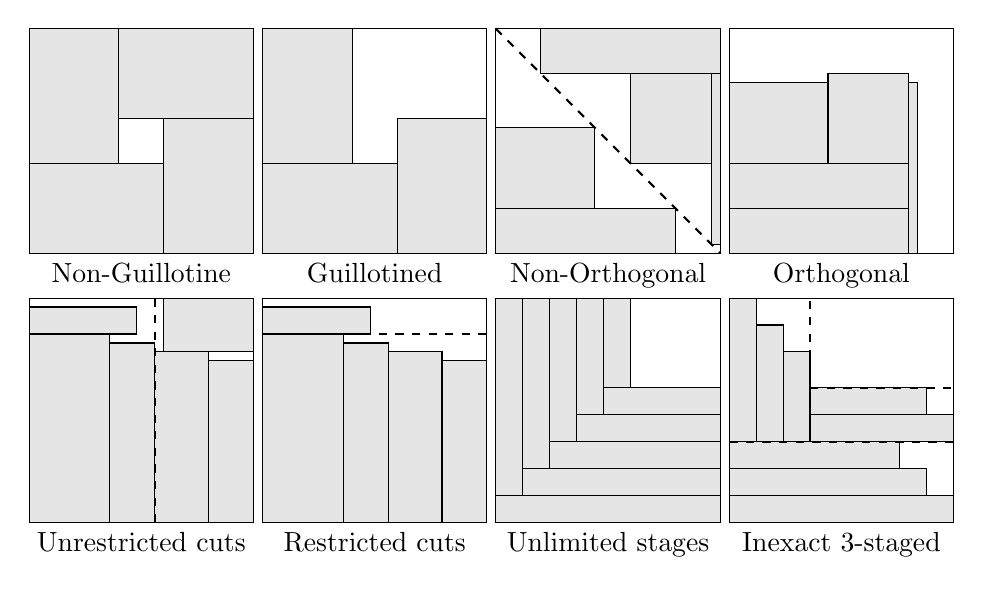
\begin{tikzpicture}[scale=0.114]
\def\piececolor{gray!20}
\def\labelxshift{12.5}
\def\labelyshift{0}
\def\labelfontsize{\normalsize}
\begin{scope}[shift={(0, 0)}] % FIRST ROW
\begin{scope}[shift={(0, 0)}] % FIRST IMAGE
\draw (0,0) rectangle +(25, 25);
\draw[fill=\piececolor] (0, 0) rectangle +(15, 10);
\draw[fill=\piececolor] (15, 0) rectangle +(10, 15);
\draw[fill=\piececolor] (0, 10) rectangle +(10, 15);
\draw[fill=\piececolor] (10, 15) rectangle +(15, 10);

\node [below] at (\labelxshift, \labelyshift) {\labelfontsize Non-Guillotine};
\end{scope}

\begin{scope}[shift={(26, 0)}] % SECOND IMAGE
\draw (0,0) rectangle +(25, 25);
\draw[fill=\piececolor] (0, 0) rectangle +(15, 10);
\draw[fill=\piececolor] (15, 0) rectangle +(10, 15);
\draw[fill=\piececolor] (0, 10) rectangle +(10, 15);
%\draw[fill=\piececolor] (10, 10) rectangle +(15, 10);

\node [below] at (\labelxshift, \labelyshift) {\labelfontsize Guillotined};
\end{scope}

\begin{scope}[shift={(52, 0)}] % THIRD IMAGE
\draw (0,0) rectangle +(25, 25);
\draw[fill=\piececolor] (0,0) rectangle +(20, 5);
\draw[fill=\piececolor] (0,5) rectangle +(11, 9);
\draw[fill=\piececolor] (5, 20) rectangle +(20, 5);
\draw[fill=\piececolor] (15, 10) rectangle +(9, 10);
\draw[fill=\piececolor] (24, 1) rectangle +(1, 19);

\draw[dashed, thick, black] (0, 25) -- (25, 0);

\node [below] at (\labelxshift, \labelyshift) {\labelfontsize Non-Orthogonal};
\end{scope}

\begin{scope}[shift={(78, 0)}] % FOURTH IMAGE
\draw (0,0) rectangle +(25, 25);
\draw[fill=\piececolor] (0,0) rectangle +(20, 5);
\draw[fill=\piececolor] (0, 10) rectangle +(11, 9);
\draw[fill=\piececolor] (0, 5) rectangle +(20, 5);
\draw[fill=\piececolor] (11, 10) rectangle +(9, 10);
\draw[fill=\piececolor] (20, 0) rectangle +(1, 19);

\node [below] at (\labelxshift, \labelyshift) {\labelfontsize Orthogonal};
\end{scope}
\end{scope}

\begin{scope}[shift={(0, -30)}] % SECOND2 ROW
\begin{scope}[shift={(0, 0)}] % FIRST IMAGE
\draw (0,0) rectangle +(25, 25);

%\draw[fill=\piececolor] (0,0) rectangle +(6, 19);
%\draw[fill=\piececolor] (6,0) rectangle +(5, 18);
\draw[fill=\piececolor] (14,0) rectangle +(6, 19);
\draw[fill=\piececolor] (20,0) rectangle +(5, 18);
\draw[fill=\piececolor] (0,0) rectangle +(9, 21);
\draw[fill=\piececolor] (9,0) rectangle +(5, 20);
%\draw[fill=\piececolor] (0,19) rectangle +(10, 6);
\draw[fill=\piececolor] (15,19) rectangle +(10, 6);
\draw[fill=\piececolor] (0,21) rectangle +(12, 3);

\draw[dashed, thick, black] (14, 0) -- (14, 25);

\node [below] at (\labelxshift, \labelyshift) {\labelfontsize Unrestricted cuts};
\end{scope}

\begin{scope}[shift={(26, 0)}] % SECOND IMAGE
\draw (0,0) rectangle +(25, 25);

%\draw[fill=\piececolor] (0,0) rectangle +(6, 19);
%\draw[fill=\piececolor] (6,0) rectangle +(5, 18);
\draw[fill=\piececolor] (14,0) rectangle +(6, 19);
\draw[fill=\piececolor] (20,0) rectangle +(5, 18);
\draw[fill=\piececolor] (0,0) rectangle +(9, 21);
\draw[fill=\piececolor] (9,0) rectangle +(5, 20);
%\draw[fill=\piececolor] (0,19) rectangle +(10, 6);
%\draw[fill=\piececolor] (15,19) rectangle +(10, 6);
\draw[fill=\piececolor] (0,21) rectangle +(12, 3);

\draw[dashed, thick, black] (0, 21) -- (25, 21);

\node [below] at (\labelxshift, \labelyshift) {\labelfontsize Restricted cuts};
\end{scope}

\begin{scope}[shift={(52, 0)}] % THIRD IMAGE
\draw (0,0) rectangle +(25, 25);

\draw[fill=\piececolor] (0,0) rectangle +(25, 3);
\draw[fill=\piececolor] (0,3) rectangle +(3, 22);
\draw[fill=\piececolor] (3,3) rectangle +(22, 3);
\draw[fill=\piececolor] (3,6) rectangle +(3, 19);
\draw[fill=\piececolor] (6,6) rectangle +(19, 3);
\draw[fill=\piececolor] (6,9) rectangle +(3, 16);
\draw[fill=\piececolor] (9,9) rectangle +(16, 3);
\draw[fill=\piececolor] (9,12) rectangle +(3, 13);
\draw[fill=\piececolor] (12,12) rectangle +(13, 3);
\draw[fill=\piececolor] (12,15) rectangle +(3, 10);

\node [below] at (\labelxshift, \labelyshift) {\labelfontsize Unlimited stages};
\end{scope}

\begin{scope}[shift={(78, 0)}] % FOURTH IMAGE
\draw (0,0) rectangle +(25, 25);
\draw[fill=\piececolor] (0,0) rectangle +(25, 3);
%\draw[fill=\piececolor] (0,3) rectangle +(3, 22);
\draw[fill=\piececolor] (0,3) rectangle +(22, 3);
%\draw[fill=\piececolor] (3,6) rectangle +(3, 19);
\draw[fill=\piececolor] (0,6) rectangle +(19, 3);

\draw[fill=\piececolor] (0,9) rectangle +(3, 16);
\draw[fill=\piececolor] (9,9) rectangle +(16, 3);
\draw[fill=\piececolor] (3,9) rectangle +(3, 13);
\draw[fill=\piececolor] (9,12) rectangle +(13, 3);
\draw[fill=\piececolor] (6,9) rectangle +(3, 10);

\draw[dashed, thick, black] (0, 9) -- (25, 9);
\draw[dashed, thick, black] (9, 9) -- (9, 25);
\draw[dashed, thick, black] (9, 15) -- (25, 15);

\node [below] at (\labelxshift, \labelyshift) {\labelfontsize Inexact 3-staged};
\end{scope}
\end{scope}
\end{tikzpicture}

\caption{Examples of valid patterns for most of the discussed problem variants. In \emph{Non-Orthogonal}, \emph{Unrestricted cuts}, and \emph{Restricted cuts}, the dashed line indicate the first cut of the pattern. In \emph{Inexact 3-staged}, the dashed line separates the three stages.}
\label{fig:qualifier_examples}
\end{figure}

While our work focuses on this specific problem, the enhanced formulation we present may be readily adapted to, at least, the Guillotine 2D version of the following problems: the Cutting Stock Problem (and the Bin Packing Problem); the Strip Packing Problem; the Multiple Knapsack Problem; the Orthogonal Packing Problem; and the variant allowing rotation for all previously mentioned problems.
See~\cite{furini:2016} for more details.
We do not define or further discuss these problems or variants in this work.

\subsection{Motivation}

\oldtext{The G2KP and its closely related variants are of undisputable interest of the industry, especially wood, paper, metal, and glass cutting industries. The vast and growing literature on the subject examined by~\cite{iori:2020} and by~\cite{russo:2020} is enough proof of such interest.
To pick a single recent case study see~\cite{clautiaux:2019}, which solves a unique variant of the Guillotine 2D Cutting Stock Problem for a glass factory manufacturing double-paned windows.}

\newtext{Guillotine cutting problems are of interest of the industry, especially the wood\cite{yanasse:linear:2008,morabito:hardboard:2007} and glass cutting industries\cite{clautiaux:2019,parreno:2020}, often because of machinery limitations. The cutting optimization problem proposed in the \emph{ROADEF/EURO Challenge 2018} was a guillotine cutting problem. The challenge was developed in collaboration with Saint-Gobain Glass France (a reference on flat glass manufacture). See~\cite{parreno:2020} for more details on this challenge. The vast and growing literature on the subject, pointed out by two recent surveys\cite{iori:2020,russo:2020}, is also evidence of such interest.}

We focus on MILP as the solving method (instead of \emph{ad hoc} solutions) because its adaptability amplifies the value of any enhancements we obtain.
\oldtext{
A better MILP formulation means:
a better solving procedure for the many (already mentioned) closely related problem variants;
a better continuous relaxation for computing an optimistic guess on the objective value of all these variants (some \emph{ad hoc} algorithms of the literature use MILP solvers to compute their bounds);
not only a better exact method but also a better base for heuristics or anytime procedures;
an immediate benefit from parallelisation, automatic problem decomposition, and solver-implemented heuristics;
and, finally, better ageing of the method over the years through the current trends of multiple-cores processors and ever-advancing solver performance.
}

\subsection{Contributions and paper outline}

The main contributions of this work are:
an enhanced MILP formulation based on a previous state-of-the-art formulation, its proof of correctness, and empirical evidence of its better performance;
a \oldtext{straigthforward}\newtext{straightforward} adaptation of a previously known reduction procedure for both the original and the enhanced formulations, and empirical evidence of its positive impact on their performance;
finally, we present new upper and lower bounds, as well as optimal values, for many recently proposed hard instances from~\cite{velasco:2019}.
For such, we reimplement a state-of-the-art MILP formulation and an optional pricing procedure used by it.
This reimplementation allows us to compare both approaches fully.
\oldtext{All code used is available in the first author's repository ({\small\url{https://github.com/henriquebecker91/GuillotineModels.jl/tree/0.2.4}}).}
\newtext{For reproducibility, the exact version of the code employed in this paper is available at~\cite{code:0:2:4}. However, we suggest using the better documented and maintained master branch ({\small\url{https://github.com/henriquebecker91/GuillotineModels.jl}}) if perfect reproduction is not necessary.}

We organise the rest of the paper the following way:
\autoref{sec:related_work} analyses how our work interacts with the pre-existing literature;
\autoref{sec:psn} introduces some mathematical concepts and explains the reduction we adapted from the literature;
\autoref{sec:enhanced_model} describes our enhanced formulation and briefly explains how it differs from the state-of-the-art formulation it is based on;
\autoref{sec:experimental_results} presents our experiments and the empirical results we derive from them;
\autoref{sec:conclusions} delivers our conclusions and suggests future work.

\section{Related work}
\label{sec:related_work}

We do not intend to provide a full overview of the literature, instead we:
refer to surveys; discuss only closely related works and how they interact with our contributions; and opportunely point out missing connections between related works.

Two relevant surveys have come out recently.
\cite{iori:2020} catalogues exact methods and relaxations for 2D cutting problems including guillotine problems.
\cite{russo:2020} reviews the literature of our particular problem at length -- there G2KP is referred to as Constrained 2D Cutting or C2DC.
Moreover, \cite{russo:2020}~points out three strategies employed by previous exact solving methods which cause loss of optimality\newtext{, i.e., these methods cannot be considered exact anymore}.
Our work does not employ any of these three strategies.
One of these strategies is a dominance rule that is valid for the unconstrained case but not for the constrained case.
In 1972, \cite{herz:1972}~proposed a dominance rule for the G2KP with unconstrained demand based on the same principle and warned about the possibility of misusing the rule in the constrained case.

The first MILP formulation dealing with guillotine cuts and unlimited stages was proposed by~\cite{messaoud:2008} in 2008.
The problem considered by~\cite{messaoud:2008} is the Strip Packing Problem\footnote{The Strip Packing Problem is a two-dimensional cutting/packing problem in which the pieces do not have profit values and the original plate does not have a predefined length (`height' in the context of the problem); the objective is to minimize the height of the original plate while packing every piece.}, but adapting the formulation to the knapsack variant would not change its fundamentals.
Previously, \cite{lodi:2003}~had proposed two MILP formulations for 2-staged G2KP.
As noted by~\cite{belov_thesis:2003}, modeling \(k\)-staged cuts for \(k \geq 3\) (unlimited stages included) was considered difficult at the time.
The size of most \(k\)-staged formulations is exponential on the number of stages (i.e.,~\(k\)).
The formulation of~\cite{messaoud:2008} had about \(3n^4/4\) variables and \(2n^4\) constraints (where \(n\) is the number of pieces) it also employed, according to the authors, a ``very loose linear relaxation'' due to which ``the practical interest of this formulation is still limited''.
The characterization of guillotine cuts proposed by~\cite{messaoud:2008} seems to have been simultaneously proposed by~\cite{pisinger:2007}. % This is the "Using decomposition" paper.

The first MILP formulation specifically for the G2KP was proposed by~\cite{furini:2016} in 2016.
An extended version of~\cite{furini:2016} appears in~\cite{dimitri_thesis} (a PhD thesis).
Their formulation has pseudo-polynomial size, \(O((L + W) \times L \times W)\)~variables and \(O(L \times W)\) constraints, and its relaxation provides a stronger bound than~\cite{messaoud:2008}.
It was the first formulation able to solve medium-sized instances of the literature.
Besides the formulation, \cite{furini:2016}~proposes two reductions and one pricing procedure; all of these are reimplemented by our work.
They also present and prove a theorem to assure the correctness of one of their reductions~(\emph{Cut-Position}).
A similar theorem and proof appear in~\cite{song:2010}.

In this work, we propose an enhanced formulation based on the one from \cite{furini:2016} mentioned above.
A significant advantage of our enhancement is to avoid the enumeration of any cuts after the middle of a plate.
This advantage appears in many works since~\cite{herz:1972}.
Recently, \cite{delorme:2019} adapted a formulation for the one-dimensional Cutting Stock Problem to obtain this same advantage.
However, the way \cite{delorme:2019}~changes their formulation to obtain this advantage is not the same as our approach.

The most recent MILP formulations for the G2KP come from three works by Martin et alii~\cite{martin:2020:models,martin:2020:bottom,martin:2020:top}.
% The formulations of~\cite{martin:2019} focus on the G2KP with defects, for which the formulation of~\cite{furini:2016} (and our enhanced version) cannot be straightforwardly adapted.
% The extra complexity needed to account for defects makes it unfair to compare their formulation against ours.
% The MILP formulations proposed in \cite{martin:2020:models,martin:2020:bottom,martin:2020:top} have the G2KP as their main target.
These formulations are compared against the formulation of~\cite{furini:2016}.
We base our enhanced formulation on~\cite{furini:2016} and also compare against it.
The formulations of ~\cite{martin:2020:models,martin:2020:bottom,martin:2020:top}
have a looser relaxation bound compared to~\cite{furini:2016}, but perform better than~\cite{furini:2016} in instances for which~\cite{furini:2016} has a much larger number of variables.
Considering the instances used in~\cite{furini:2016}, our enhanced formulation dominates the formulation of~\cite{furini:2016}.
Our formulation also dramatically improves the running times of instances in which the formulation of~\cite{furini:2016} performed worse than \cite{martin:2020:models,martin:2020:bottom,martin:2020:top} (e.g., the gcut1--gcut12 instances).
Consequently, while it may be interesting for completeness sake, we do not compare against the formulations proposed in~\cite{martin:2020:models,martin:2020:bottom,martin:2020:top}.

% We discuss the related works in the topic of cut position discretization in the following section.
% The topic demands more notation and connects with the reduction we adapt from the previous literature for our enhanced formulation.

% TODO: Should all words in the title be capitalized?
% TODO: Is this title ok? maybe Normalizing Plate Size?
\section{Notation, Discretization, and Plate-Size Normalization}
\label{sec:psn}

The performance of solving methods for cutting and packing problems often heavily depends on the number of (cut/packing) positions considered.
Since the seminal works of~\cite{nicos:1977} and~\cite{herz:1972}, solving methods avoid considering each possible position, but instead consider only a subset necessary to guarantee optimality.
The literature includes many such subsets, which are often referred to as \emph{discretizations}.
The most common way of computing these discretizations are Dynamic Programming (DP) algorithms.
These DP algorithms usually only take a small fraction of the running time, but the size of the position subset outputted by them strongly affects the time spent by the rest of the solving method.

Both~\cite{furini:2016} and our enhanced formulation have one constraint for each attainable distinctly-sized plate and one variable for each potential cut over each of these plates.
Therefore, eliminating a single cutting position has the following effects:
\textbf{(i)} it removes one variable for each distinctly-sized plate that allowed that cutting position;
\textbf{(ii)} if that cutting position was the only way to produce some distinctly-sized plates\footnote{Note that the same cutting position, when applied to distinctly-sized plates, may generate different children.}, then it also removes the constraints associated with these plates;
\textbf{(iii)} if (ii) excludes one or more constraints/plates, then it also excludes all variables representing possible cuts over the excluded plates;
\textbf{(iv)} finally, if (iii) eliminates one or more variables/cuts, then it may trigger (ii) again (i.e., other plates stop being attainable), cyclically.

In this work, the only cut subset (discretization) considered are the canonical dissections of~\cite{herz:1972}, hereafter referred to as \emph{normal cuts} instead.
We acknowledge the existence of stricter discretizations: the raster points of~\cite{terno:1987,guntram:1966}, the regular normal patterns of~\cite{boschetti:2002} (named this way by~\cite{cote:2018}), and the Meet-in-the-Middle (MiM) of~\cite{cote:2018}.
The reasons for our choice of discretization are numerous:
it works well with the \emph{Plate-Size Normalization} procedure we describe below;
it is the same discretization employed by~\cite{furini:2016} (from which we base our enhanced formulation on);
\oldtext{MiM main gain}\newtext{The main gain of MiM} is reducing the number of cut positions after the middle of a plate, which our enhanced formulation already discards anyway;
the regular normal patterns compute a distinct subset-sum for each pair of plate and piece, which we consider excessive (there may exist hundreds of thousands of intermediary plate possibilities);
finally, the raster points complicate our proofs and our \emph{Plate-Size Normalization} weakens its benefits.

The set~\(O = \{v, h\}\) denotes the cut orientation: \(v\) is vertical (parallel to \oldtext{width}\newtext{length}, \oldtext{perpedicular}\newtext{perpendicular} to \oldtext{length}\newtext{width}); \(h\) is horizontal (parallel to \oldtext{length}\newtext{width}, perpendicular to \oldtext{width}\newtext{length}).
Let us recall that the demand of a piece~\(i \in \bar{J}\) is denoted by~\(u_i\).
If we define the set of pieces fitting a plate~\(j\) as~\(I_j = \{i \in \bar{J} : l_i \leq l_j \land w_i \leq w_j \}\), we can define~\(N_{jo}\) (i.e., the set of the normal cuts of orientation~\(o\) over plate~\(j\)) as:

{\iffinalversion\else\color{blue}\fi
\begin{equation}
N_{jo}= \left\{
\begin{array}{lllr}
  \{q: 0 < q < l_j; & \exists n_i \in [0 \isep u_i], \forall i \in I_j, q = \sum_{i\in I_j} n_i l_i \} & \quad \text{if } o = h,\\
  \{q: 0 < q < w_j; & \exists n_i \in [0 \isep u_i], \forall i \in I_j, q = \sum_{i\in I_j} n_i w_i \} & \quad \text{if } o = v.
\end{array}\right.
\end{equation}
}

The sets defined above never include cuts at the plate extremities (i.e., \(0\), \(l_j\) for \oldtext{\(N_{jv}\)}\newtext{\(N_{jh}\)}, and \(w_j\) for \oldtext{\(N_{jh}\)}\newtext{\(N_{jv}\)}).
Any of these cuts will always create (i)~a~zero-area plate and (ii)~a~copy of the plate that is being cut.
Consequently, these cuts only add symmetries and may be disregarded.

\newtext{The set \(J\) can now be defined by the following procedure: the original plate (plate~\(0\)) is added to \(J\), then for every plate~\(j \in J\) every cut in~\(N_{jv} \cup N_{jh}\) is applied to~\(j\), and each child generated is added to \(J\) if it can fit at least one piece. The process finishes when every plate in~\(J\) was considered for cutting, and no new plates were generated. Such procedure guarantees each piece~\(i \in \bar{J}\) will always be present in~\(J\) unless the piece does not fit the original plate (in which case it is irrelevant to the problem and could be removed a priori).}

The goal of the \emph{Plate-Size Normalization} procedure we propose is to reduce the number of distinctly-sized plates considered.
Fewer distinctly-sized plates mean fewer constraints and trigger the same cascading effect described by items (ii)--(iv) above.
The property exploited by the procedure is already known and similarly exploited by~\cite{alvarez:2009} and by~\cite{dolatabadi:2012}.
We state the property as:

\begin{proposition}
\label{pro:normalization}
% Without loss of optimality, plate~\(j\) may always be replaced by plate~\(j\prime\) with \(w_{j\prime} = w_j\) but \(l_{j\prime} = max\{q : q \in N_{kv}, q \leq l_j\}\) in which \(w_k = w_j\) but \(l_k > l_j\).
Given a plate~\(j \in J\), \(l_j\) may always be replaced by \(l^\prime_j = max\{q : q \in\) \oldtext{\(N_{kv}\)}\newtext{\(N_{kh}\)}\(, q \leq l_j\}\) in which \(k \in J\), \(w_k = w_j\), but \(l_k > l_j\), without loss of optimality.
The analogue is valid for the width.
\end{proposition}

\newtext{In other words, if increasing the length (width) of plate~\(j\) reveals that the original length (width) did not match a normal cut position in the enlarged plate, then plate~\(j\) may be replaced by a shorter plate in which the length (width) is reduced to the largest normal cut position smaller than the original length (width). For example, given \(l = [5, 7]\), \(w = [3, 2]\), a 13x3 plate may be reduced to 12x3 (13 does not match a normal cut while \(5 + 7 = 12\) does), and a 13x2 plate may be reduced to 7x2 (13 does not match a normal cut while 7 does).}
We do not replicate any proof here. We can then define:

\begin{definition}
The length of a plate~\(j\) is considered normalized if, and only if, \(l_j = l^\prime_j\).
The analogue is valid for the width.
The size of a plate is normalized if, and only if, both its length and its width are normalized.
\end{definition}

The \emph{Plate-Size Normalization} procedure we propose consists only of replacing every non-size-normalized plate enumerated by their normalized counterpart.
The number of distinctly-sized plates diminishes because the procedure replaces many plates of distinct but similar dimensions by a single plate.
The only extra effort added by \emph{Plate-Size Normalization} consists of binary searches over~\(N_{jo}\) sets for each plate~\(j\)\newtext{, and these may be carried out without increasing the overall complexity, given the setup of~\(O(LW)\) vectors of size \(O(L + W)\); a setup step which also does not increase the overall complexity. However, in our implementation, we opted to increase the overall complexity from \(O(L^2W + LW^2)\) to \(O(L^2Wlog(L) + LW^2log(W))\) because the fraction of time spent on the enumeration was not enough to justify the memory and code complexity trade-off. In practice, even if our worst-case complexity increases, the time spent decreased because the actual number of plates (denoted in the complexity by~\(O(LW)\) became more distant from the worst-case}.
A suitable \(N_{ko}\) set for each plate~\(j\) was already computed by the plate enumeration procedure before introducing the \emph{Plate-Size Normalization} (no extra effort required).

\begin{remark}
\oldtext{If a normal cut~\(q\) divides the size-normalized plate~\(j\), the first child is always size normalized, but the second child may not be size normalized.}
\newtext{If a normal cut divides a size-normalized plate, then the dimension perpendicular to the cut, in the first child, is normalized. The dimension parallel to the cut in the first child, and both dimensions of the second child, are not guaranteed to be normalized.}
\end{remark}

% Every optimal solution with non-normal cuts can be mapped to an optimal solution only using normal cuts.
% The definition used here is almost the same of~\cite{furini:2016}, as we are trying to keep our notation compatible with theirs.

% TODO: the definitions below need the definition of orientation.
% TODO: define the sizes set `S_{oj}` where? "given vertical cuts are parallel to length and horizontal cuts parallel to width, we define the size set ..."
% TODO: define Q_{jo} here, like in furini:2016, maybe change paragraph above to say we will be using the same definition of furini:2016

% is the set of pieces that fit plate~\(j\).
%\(O = \{v, h\}\) defines both vertical and horizontal orientations.
%Considering that vertical is parallel to length, and horizontal is parallel to width, we can use them to index plate sizes as in~\(S_{jv} = l_j\) and \(S_{jh} = w_j\).
%Allowing us to define normal cuts as:

%\begin{definition}
%\(Q_{jo} = \{ 0 < q < S_{oj}; \forall i \in I_j, \exists n_i \in \mathbb{N}, n_i \leq u_i, q = \sum_{i\in I_j n_i S_{oi}}\}\)
%\end{definition}

% Let us denote the \emph{original plate} as plate~\(0\).
% Every cut c in Q_{0o} define a plate with a side of size S_{0o} and another of size S_{co}


% The \emph{plate-size normalization} works by replacing groups of plates (with similar but distinct size) by a single plate.
% If there exists a plate~\(j : S_{oj} > max\{N_{oj}\}\) then \(j\) may be replaced by a plate~\(k : S_{ok} = max\{N_{oj}\}\).
% 

%In this section, we prove that no valid solution is lost if plate dimensions are shortened to a discretization point.
%For convenience, we denote the set of pieces that fit a plate~\(j\) by \(\bar{J}_j\); a piece~\(i\) fits a plate~\(j\) iff \(l_i \leq L_j \land w_i \leq W_j\).%, and that plates cut from a shortened plate may need additional shortening after the cut.

%\begin{definition}
%The set of pieces that fit a plate~\(j\) is denoted by \(\bar{J}_j\), a piece~\(i\) fit a plate~\(j\) if \(l_i \leq L_j \land w_i \leq W_j\).
%\end{definition}

%\begin{definition}
%The set of horizontal normal cuts of a plate~\(j\) is the set of all non-trivial linear combinations \(\sum_{i \in \bar{J}_j} a_i \times l_i \leq L\) for which the coefficients \(a_i\) are restricted by \(0 \leq a_i \leq u_i~\forall.~i \in \bar{J}_j\). The analogue is valid for vertical cuts.
%\end{definition}

%In~\cite{nicos:1977}, \emph{normal cuts} are defined for the variant of the problem without the demand constraints.
%Our definition of normal cuts is extended to take into consideration the demand.
%The following theorem and its proof (provided in \autoref{app:proof_only_normal_cuts_needed}) are also extensions to account for the demand.
%We also extend a theorem, and its proof, that restricting the cuts to (our definition of) normal cuts allows packing any demand-abiding piece mulstiset that could be packed with non-normal cuts.
%We also extend a theorem, and its proof, that restricting the cuts to (our definition of) normal cuts allows packing any demand-abiding piece mulstiset that could be packed with non-normal cuts.

%\begin{theorem}\label{only_normal_cuts_needed}
%For every guillotine packing with non-normal cuts packing a set of pieces~\(s\), there is a guillotine packing of only normal cuts packing the largest subset of~\(s\) that respects the demand.
%producing the same pieces or, if the former packing produced an amount exceeding the demand for some piece type, the latter paproduces the maximum amount allowed by the demand for such piece types.
%\end{theorem}

%is in the appendix, as similar proofs are presented in the literature.

%\begin{corollary}\label{co:size_normalized_plate}
%Given a plate~\(j\) in which the right (or top) border do not overlap with the rightmost vertical (or topmost horizontal) normal cut, any demand-abiding piece multiset packed in~\(j\) can be packed in its size-normalized alternative, in which the plate size is reduced until the borders overlap with normal cuts.
%\end{corollary}

%\begin{proof}
%The proof of the~\autoref{only_normal_cuts_needed} describes an alternative packing with the property that any space between the rightmost vertical cut and the plate right border (topmost horizontal cut and the plate top border) is waste. Therefore, if a plate is replaced by its size-normalized alternative, no used space would be lost, and no packing would be invalid.\qed
%\end{proof}

%\begin{remark}
%If a size-normalized plate is cut by a normal cut, the first child is also size-normalized. The second child, however, may or may not be size-normalized.
%\end{remark}

%In the dimension parallel to the cut, the border of the first child will overlap with the normal cut applyed to the parent plate; on the other dimension, the border already overlapped a normal cut.

\begin{example}\label{ex:renormalization_after_cut}
\oldtext{Given two pieces with \(l = [5, 7]\), \(u = [2, 3]\), and a size-normalized plate of length~\(21\), a normal cut at~\(12\) creates a non-normalized second child of length~ \(9\).}
\newtext{Consider three pieces with~\(l = [5, 7, 9]\), \(w = [6, 4, 11]\), \(u = [3, 1, 1]\), and a plate of dimensions \(15\)x\(15\). The plate dimensions are already normalized. The plate length matches stacking the three copies of the first piece. The plate width matches laying side-by-side the other two pieces. An horizontal cut at length~\(7\) is a normal cut because it matches the length of the second piece. If the cut is done, the width of both children is not normalized anymore, nor is the length of the second child. The width of both children is not normalized because the third piece does not fit either child so, for both children, the largest width a valid packing may reach is~\(12\). The length of the second child is not normalized because the largest length a valid packing inside the second child may reach is 7. The dimensions of both children may be normalized to \(7\)x\(12\). This example already shows an immediate gain, instead of creating two new plate sizes, the enumeration only creates a single new plate type. The cut creates two copies of this single type of plate.}
\end{example}

\begin{figure}
\center
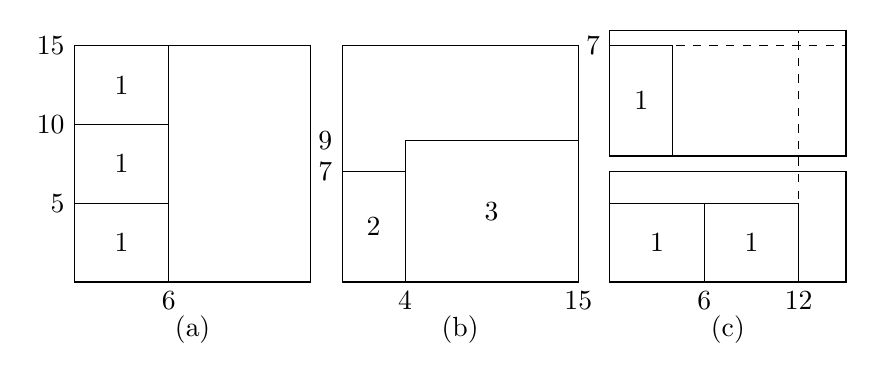
\begin{tikzpicture}[scale=0.20]
\begin{scope}[shift={(0, 0)}]
\draw [draw=black]   (0, 0) rectangle ++(15, 15);
\draw [draw=black]   (0, 0) rectangle     ++(6, 5) node [midway] {1};
\draw [draw=black]   (0, 5) rectangle     ++(6, 5) node [midway] {1};
\draw [draw=black] (0, 10) rectangle     ++(6, 5) node [midway] {1};
\node [left]  at (0, 5) {5};
\node [left]  at (0, 10) {10};
\node [left]  at (0, 15) {15};
\node [below]  at (6, 0) {6};
\node [below] at (7.5, -1.5) {(a)};
\end{scope}
\begin{scope}[shift={(17, 0)}]
\draw [draw=black]   (0, 0) rectangle ++(15, 15);
\draw [draw=black]   (0, 0) rectangle     ++(4, 7) node [midway] {2};
\draw [draw=black]   (4, 0) rectangle   ++(11, 9) node [midway] {3};
\node [below]  at   (4, 0)   {4};
\node [below]  at (15, 0) {15};
\node     [left]  at   (0, 7)   {7};
\node   [left]  at (0, 9)   {9};
\node [below] at (7.5, -1.5) {(b)};
\end{scope}
\begin{scope}[shift={(34, 0)}]
\draw [draw=black]   (0, 0) rectangle ++(15, 7);
\draw [draw=black]   (0, 0) rectangle     ++(6, 5) node [midway] {1};
\draw [draw=black]   (6, 0) rectangle     ++(6, 5) node [midway] {1};
\node [below]  at (6, 0) {6};
\node [below]  at (12, 0) {12};
\draw[dashed] (12, 0) -- (12, 16);

\draw [draw=black]   (0, 8) rectangle ++(15, 8);
\draw [draw=black]   (0, 8) rectangle   ++(4, 7) node [midway] {1};

\node     [left]  at   (0, 15)   {7};
\draw [dashed] (0, 15) -- (15, 15);
\node [below] at (7.5, -1.5) {(c)};
\end{scope}
\end{tikzpicture}
\caption{\newtext{Diagram of~\cref{ex:renormalization_after_cut}: (a) the three copies of the first piece stacked; (b) the second and third pieces side-by-side; (c) both children of a horizontal normal cut over a normalized plate are not normalized themselves.}}
\label{fig:renormalization_after_cut}
\end{figure}

\begin{comment}
\subsection{Expanded example for thesis proposal}

I need an original plate and about 3~5 pieces.
Ideally the original plate should already be size-normalized, to be fair.
The smallest piece needs to be distant of one in absolute terms, but cannot be on the relatively large side, because this makes harder for an intermediary plate have many replacements.
We may use only squares, but this is kinda boring.
Probably the easiest way is to make a branch of the code in which the code enumerating plates saves which non-normalized plates were replaced by each normalized plate and outputs them.
\end{comment}

\section{Our changes to Furini's model}
\label{sec:enhanced_model}

% NEED TO DEFINE:
% Q_{jo} as the subset of the linear combinations for some plate and orientation
% in the original paper the only cuts removed are the symmetric ones, in our
% case we remove all after midplate
% we also make use of the corollary in last section to reduce the number of
% plates considered, what consequently reduces the number of variables
% * such sacrifice allows to remove some symmetries with a simpler method than redundant-cuts but, most importantly, it allows us to remove a large number of cut variables by inserting a lower number of extraction variables
% * there is a typo on the definition of 'a' at the source (say this after explaining coefficient a)

The formulation proposed in~\cite{furini:2016} is elegant: the pieces are just intermediary plates that may be sold.
Our contribution consists of changes to both the preprocessing step and to the formulation.
These changes significantly reduce the number of variables.
Differently, these changes deepen the distinction between plates and pieces and, consequently, may be regarded as sacrificing some elegance for performance.
The essentials of the formulation remain the same and, for this reason, we consider the model presented here as an enhanced model, not an entirely new model.

% TODO: should we say that this supersedes the furini original symm-breaking
% and their redundant-cut reduction?

The cut enumeration in~\cite{furini:2016} excludes some symmetric cuts; that is, if two different cuts create the same set of two child plates, then the symmetric cut in the second half of the plate may be ignored.
Differently,~\cite{nicos:1977} disregards \emph{all} cuts after the middle of the plate because of symmetry.
If~\cite{furini:2016} would do the same as~\cite{nicos:1977} it could become impossible to trim a plate to the size of a piece.
For example, if there was a piece with length larger than half the length of a plate, and such plate has no normal cut with the exact length of the needed trim, then the piece could not be extracted from the plate, even if the piece fits the plate.
The goal of our changes is to reduce the number of cuts (i.e., model variables) by getting closer to the symmetry-breaking rule used in~\cite{nicos:1977} without loss of optimality.
%First we present our changes to the formulation and the variable enumeration, then we prove the model correctness is not affected.

%Often, there are many more normal cuts in the second half of a plate than there is in the first half. % need explanation?
%Also, if all cuts that generated some plate type are disregarded, then every cut over such plate type is also disregarded.
%Taking all of this into account, the main purpose of our revised version of Furini's formulation is to improve its symmetry breaking. % TODO: This has also the effect of superseding the Redundant-Cut reduction, which EXPLAIN SUCCINTLY THE REDUNDANT CUT.

\subsection{The enhanced formulation}
\label{sec:enhanced}

Our changes to the formulation are restricted to replacing the set of integer variables~\(y_j, i \in \bar{J},\) with a new set of variables~\(e_{ij}, (i, j) \in E, E \subseteq \bar{J} \times J\), and the necessary adaptations to accomodate this change.
In the original formulation, \(y_i\) denoted the number of times a plate~\(i\) was sold as the piece~\(i\), in this case, the plate always had the exact size of the piece.
Our \emph{extraction variables}~\(e_{ij}\) denote a piece~\(i\) was extracted from plate~\(j\), which size may differ from the size of the piece.
\newtext{The exact definition of set~\(E\) is discussed over~\autoref{sec:var_enum}; for the purpose of presenting the formulation, our intuitive definition of~\(e_{ij}\) just above is enough.}
For convenience, we also define \(E_{i*} = \{ j : \exists~(i, j) \in E \}\) and \(E_{*j} = \{i : \exists~(i, j) \in E \}\).
The set \(O = \{h, v\}\) denotes the horizontal and vertical cut orientations.
The set \(Q_{jo}\) (\(\forall j \in J, o \in O\)) denotes the set of possible cuts (or cut positions) of orientation~\(o\) over plate~\(j\).

The parameter~\(a\) is a byproduct of the plate enumeration process.
\oldtext{If cutting a plate~\(k \in J\) with a cut of orientation~\(o \in O\) at position~\(q \in Q_{jo}\) adds a plate~\(j \in J\) to the stock, then~\(a^o_{qkj} = 1\); otherwise~\(a^o_{qkj} = 0\).}
\newtext{The value of~\(a^o_{qkj}\) indicates how many copies of a plate~\(j \in J\) are produced by cutting a plate~\(k \in J\) with a cut of orientation~\(o \in O\) at position~\(q \in Q_{ko}\).}
%This parameter is needed to write the constraint that control which plates are available.
The description of this parameter in~\cite{furini:2016} has a typo, as pointed out by~\cite{martin:2020}:
``[...] there is a typo in their definition of parameter~\(a^o_{qkj}\), as the indices~\(j\) and~\(k\) seem to be exchanged.''.

In a valid solution, the value of \(x^o_{qj}\) is the number of times a plate~\(j \in J\) is cut with orientation~\(o \in O\) at position~\(q \in Q_{jo}\); while the value of~\(e_{ij}\) is the number of sold pieces of type~\(i \in \bar{J}\) that were extracted from plates of type~\(j \in J\).
The plate~\(0 \in J\) is the original plate, and it may also be in~\(\bar{J}\), as there may exist a piece of the same size as the original plate.

%\hspace*{\fill}
\begin{align}
\mbox{max.} &\sum_{(i, j) \in E} p_i e_{ij} \label{eq:objfun}\\
\mbox{s.t.} &\sum_{o \in O}\sum_{q \in Q_{jo}} x^o_{qj} + \sum_{i \in E_{*j}} e_{ij} \leq \sum_{k \in J}\sum_{o \in O}\sum_{q \in Q_{ko}} a^o_{qkj} x^o_{qk} \hspace*{0.05\textwidth} & \forall j \in J, j \neq 0,\label{eq:plates_conservation}\\
%	& \specialcell{\sum_{o \in O}\sum_{q \in Q_{jo}} x^o_{qj} \leq \sum_{k \in J}\sum_{o \in O}\sum_{q \in Q_{ko}} a^o_{qkj} x^o_{qk} \hspace*{\fill} \forall j \in J\setminus\bar{J},}\label{eq:generic_plates_conservation}\\
	& \sum_{o \in O}\sum_{q \in Q_{0o}} x^o_{q0} + \sum_{i \in E_{*0}} e_{i0} \leq 1 &,\label{eq:just_one_original_plate}\\
	& \sum_{j \in E_{i*}} e_{ij} \leq u_i & \forall i \in \bar{J},\label{eq:demand_limit}\\
% TODO: fix equation below, the forall part is too long and clashes with the long equation in the first line
	& x^o_{qj} \in \mathbb{N}^0 & \forall j \in J, o \in O, q \in Q_{jo},\label{eq:trivial_x}\\
	& e_{ij} \in \mathbb{N}^0 & \forall (i, j) \in E.\label{eq:trivial_e}
\end{align}

The objective function maximizes the profit of the extracted pieces~\eqref{eq:objfun}.
Constraint~\eqref{eq:plates_conservation} guarantees that for every plate~\(j\) that was further cut or had a piece extracted from it (left-hand side), there must be a cut making available a copy of such plate (right-hand side).
One copy of the original plate is available from the start~\eqref{eq:just_one_original_plate}.
The amount of extracted copies of some piece type must respect the demand for that piece type (a piece extracted is a piece sold)~\eqref{eq:demand_limit}.
Finally, the domain of all variables is the non-negative integers~\eqref{eq:trivial_x}-\eqref{eq:trivial_e}.

\subsection{The revised variable enumeration}
\label{sec:var_enum}

The variable enumeration described in~\cite{furini:2016} employs some rules to reduce the number of variables; they are symmetry-breaking, \emph{Cut-Position}, and \emph{Redundant-Cut}.
The two last rules are not discussed here; \cite{furini:2016}~proves their correctness and they do not conflict with the enhanced model.

The use of the \(x\)~variables does not change from the original formulation to our revised formulation -- however, the size of the enumerated set of variables changes.
Our revised enumeration does not create any variable~\(x^o_{jq}\) in which \((o = h \land q > \lceil w_j / 2 \rceil) \lor (o = v \land q > \lceil l_j / 2 \rceil)\).
%given that \(D^h_j \equiv W_j\) and \(D^v_j \equiv L_j\).

The original formulation has variables~\(y_i\), \(i \in \bar{J}\), while the revised formulation replaces them with variables~\(e_{ij}\), \((i, j) \in E\), \(E \subseteq \bar{J} \times J\).
Set~\(\bar{J} \times J\) is orders of magnitude larger than~\(\bar{J}\).
Consequently, set~\(E\) must be a small subset to avoid having a revised model with more variables than the original.
A suitable subset may be obtained by a simple rule: \((i, j) \in E\) if, and only if, packing piece~\(i\) in plate~\(j\) does not allow any other piece to be packed in~\(j\).

\newtext{For the enhanced formulation to have more variables than the original formulation, \(|E| > |\bar{J}| + |\{x^o_{jq} : j \in J \land o \in O \land q \in Q_{jo} \land (o = h \land q > \lceil w_j / 2 \rceil) \lor (o = v \land q > \lceil l_j / 2 \rceil)\}|\) must hold, this is, the number of extraction variables must be larger than the number of pieces plus the sum of the number of cuts after the middle of each enumerated plate. Unfortunately, there is no closed formula for these sets (except \(\bar{J}\) which is given), what makes necessary to compute the full enumeration to verify the difference.}


%The reason this restricted subset is enough to keep the model correctness is presented in next section.

%If an extra piece could be packed, then there is a normal cut that creates both a plate that may be used for this extra piece and a plate that may be used to pack~\(i\).
%So the idea here is to do the extraction as late as possible: if the piece may be extracted from a descendant, then the plate may be cut until this descendant is generated to then have the piece extracted from it.

\subsection{The proof of correctness}
\label{sec:proof_of_correctness}

The previous section presented a detailed explanation of the changes to the formulation and variable enumeration.
This section proves such changes do not affect the correctness of the model.
In~\cite{furini:2016}, only the perfect symmetries described below are removed.
Our changes may be summarized to:

\begin{enumerate}
\item There is no variable for any cut that occurs after the middle of a plate.
\item A piece may be obtained from a plate if, and only if, the piece fits the plate, and the plate cannot fit an extra piece (of any type).
\end{enumerate}

The second change alone cannot affect the model correctness.
The original formulation was even more restrictive in this aspect:
a piece could only be sold if a plate of the same dimensions existed.
In our revised formulation there will always exist an extraction variable in such case:
if a piece and plate match perfectly, there is no space for any other piece, fulfilling our only criteria for the existence of extraction variables.
Consequently, what needs to be proved is that:

\begin{theorem}
\label{the:enhanced_correctness}
Without changing the pieces obtained from a packing, we may replace any normal cut after the middle of a plate by a combination of piece extractions and cuts at the middle of a plate or before it.
\end{theorem}

%Both the theorem above and the proof below assume a plate cannot be cut twice.
%If a single cut is applied to a plate, then two new plates are created, and these may be further cut.
%There is no loss of generality by undertaking this assumption, it is just the difference between representing the packing by a binary tree, instead of tree with a variable number of children.

\begin{proof}
This is a proof by exhaustion. The set of all normal cuts after the middle of a plate may be split into the following cases:
\begin{enumerate}
  \item The cut has a perfect symmetry. \label{case:perfectly_symmetric}
  \item The cut does not have a perfect symmetry.
  \begin{enumerate}
    \item Its second child can fit at least one piece. \label{case:usable_second_child}
    \item Its second child cannot fit a single piece.
    \begin{enumerate}
      \item Its first child packs no pieces. \label{case:no_pieces}
      \item Its first child packs a single piece. \label{case:one_piece} % call luffy to help
      \item Its first child packs two or more pieces. \label{case:many_pieces}
    \end{enumerate}
  \end{enumerate}
\end{enumerate}

We believe to be self-evident that the union of~\cref{case:perfectly_symmetric,case:usable_second_child,case:no_pieces,case:one_piece,case:many_pieces} is equal to the set of all normal cuts after the middle of a plate. We present an individual proof for each of these cases.


\begin{description}
\item[\Cref{case:perfectly_symmetric} -- \textbf{The cut has a perfect symmetry.}]
If two distinct cuts have the same children (with the only difference being the first child of one cut is the second child of the other cut, and vice-versa), then the cuts are perfectly symmetric.
Whether a plate is the first or second child of a cut does not make any difference for the formulation or for the problem.
If the cut is in the second half of the plate, then its symmetry is in the first half of the plate.
Consequently, both cuts are interchangeable, and we may keep only the cut in the first half of the plate.
\item[\Cref{case:usable_second_child} -- \textbf{Its second child can fit at least one piece.}]
\autoref{pro:normalization} allows us to replace the second child by a size-normalized plate that can pack any demand-abiding set of pieces the original second child could pack.
The second child of a cut that happens after the middle of the plate is smaller than half a plate, and its size-normalized counterpart may only be the same size or smaller.
So the size-normalized plate could be cut as the first child by a normal cut in the first half of the plate.
Moreover, the old first child (now second child) have stayed the same size or grown (because the size-normalization of its sibling), which guarantee this is possible.

\item[\Cref{case:no_pieces} -- \textbf{Its first child packs no piece.}]
If both children of a single cut do not pack any pieces, then the cut may be safely ignored.
\item[\Cref{case:one_piece} -- \textbf{Its first child packs a single piece.}]
First, let us ignore this cut for a moment and consider the plate being cut by it (i.e., the parent plate).
The parent plate either: can fit an extra piece together with the piece the first child would pack, or cannot fit any extra pieces.
If it cannot fit any extra pieces, this fulfills our criteria for having an extraction variable, and the piece may be obtained through it.
The cut in question can then be disregarded (i.e., replaced by the use of such extraction variable).
However, if it is possible to fit another piece, then there is a normal cut in the first half of the plate that would separate the two pieces, and such cut may be used to shorten the plate.
This kind of normal cuts may successively shorten the plate until it is impossible to pack another piece, and the single piece that was originally packed in the first child may then be obtained employing an extraction variable.
\item[\Cref{case:many_pieces} -- \textbf{Its first child packs two or more pieces.}]
If the first child packs two or more pieces, but the second child cannot fit a single piece (i.e., it is waste), then the cut separating the first and second child may be omitted and any cuts separating pieces inside the first child may still be done.
If some of the plates obtained by such cuts need the trimming that was provided by the omitted cut, then these plates will be packing a single piece each, and they are already considered in~\cref{case:one_piece}.
\end{description}

Given the cases cover every cut after the middle of a plate, and each case has a proof, then follows that \Cref{the:enhanced_correctness} is correct. \qed
\end{proof}

\begin{figure}
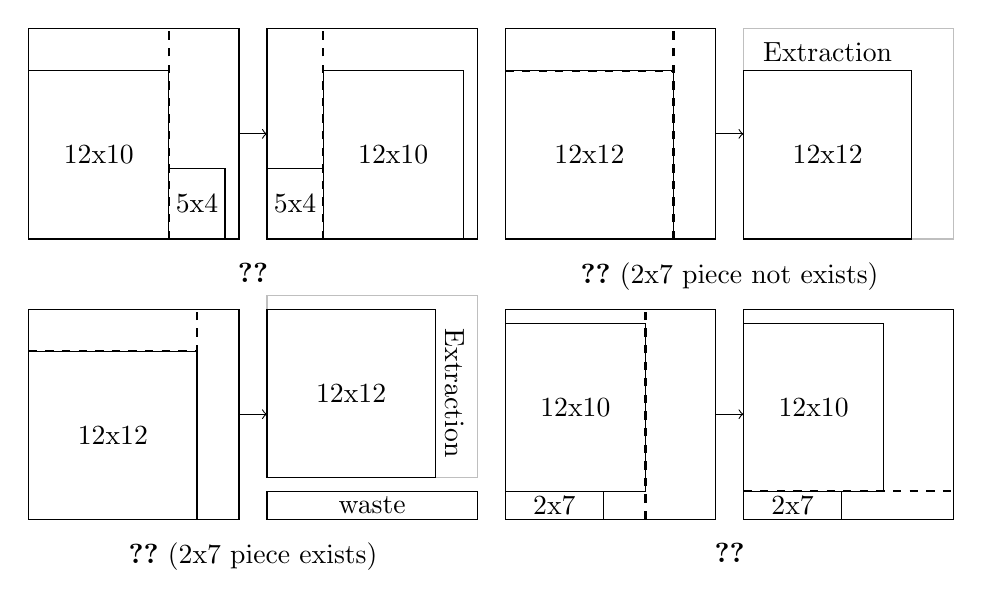
\begin{tikzpicture}[scale=0.178]
\def\piececolor{gray!20}
\def\labelxshift{16}
\def\labelyshift{-1}
\def\labelfontsize{\normalsize}
\def\innerlabelfontsize{\normalsize}
\def\extractioncolor{gray!50}
\begin{scope}[shift={(0, 0)}] % FIRST ROW
\begin{scope}[shift={(0, 0)}] % FIRST PAIR
\begin{scope}[shift={(0, 0)}] % FIRST IMAGE
\draw (0,0) rectangle +(15, 15);
\draw (0, 0) rectangle +(10, 12) node [midway] {\innerlabelfontsize 12x10};
\draw (10, 0) rectangle +(4, 5) node [midway] {\innerlabelfontsize 5x4};

\draw[dashed, thick, black] (10, 0) -- (10, 15);
\draw [-to](15, 7.5) -- (17,7.5);
\end{scope} % FIRST IMAGE

\begin{scope}[shift={(17, 0)}] % SECOND IMAGE
\draw (0,0) rectangle +(15, 15);
\draw (4, 0) rectangle +(10, 12) node [midway] {\innerlabelfontsize 12x10};
\draw (0, 0) rectangle +(4, 5) node [midway] {\innerlabelfontsize 5x4};

\draw[dashed, thick, black] (4, 0) -- (4, 15);
\end{scope} % SECOND IMAGE

\node [below] at (\labelxshift, \labelyshift) {\labelfontsize \Cref{case:usable_second_child}};
\end{scope} % FIRST PAIR


\begin{scope}[shift={(34, 0)}] % SECOND PAIR
\begin{scope}[shift={(0, 0)}] % FIRST IMAGE
\draw (0,0) rectangle +(15, 15);
\draw (0, 0) rectangle +(12, 12) node [midway] {\innerlabelfontsize 12x12};

\draw[dashed, thick, black] (12, 0) -- (12, 15);
\draw[dashed, thick, black] (0, 12) -- (12, 12);
\draw [-to](15, 7.5) -- (17,7.5);
\end{scope} % FIRST IMAGE

\begin{scope}[shift={(17, 0)}] % SECOND IMAGE
\draw[draw=gray!50] (0,0) rectangle +(15, 15);
\node [above] at (6, 12) {\labelfontsize Extraction};
\draw (0, 0) rectangle +(12, 12) node [midway] {\innerlabelfontsize 12x12};
\end{scope} % SECOND IMAGE

\node [below] at (\labelxshift, \labelyshift) {\labelfontsize \Cref{case:one_piece} (2x7 piece not exists)};
\end{scope} % SECOND PAIR
\end{scope} % FIRST ROW



\begin{scope}[shift={(0, -20)}] % SECOND ROW
\begin{scope}[shift={(0, 0)}] % FIRST PAIR
\begin{scope}[shift={(0, 0)}] % FIRST IMAGE
\draw (0,0) rectangle +(15, 15);
\draw (0, 0) rectangle +(12, 12) node [midway] {\innerlabelfontsize 12x12};

\draw[dashed, thick, black] (12, 0) -- (12, 15);
\draw[dashed, thick, black] (0, 12) -- (12, 12);
\draw [-to](15, 7.5) -- (17,7.5);
\end{scope} % FIRST IMAGE

\begin{scope}[shift={(17, 0)}] % SECOND IMAGE
\node [rotate=-90, above] at (12, 9) {\labelfontsize Extraction};
\draw[draw=\extractioncolor] (0, 3) rectangle +(15, 13);

\draw (0, 0) rectangle +(15, 2) node [midway] {waste};

\draw (0, 3) rectangle +(12, 12) node [midway] {\innerlabelfontsize 12x12};
\end{scope} % SECOND IMAGE

\node [below] at (\labelxshift, \labelyshift) {\labelfontsize \Cref{case:one_piece} (2x7 piece exists)};
\end{scope} % FIRST PAIR


\begin{scope}[shift={(34, 0)}] % SECOND PAIR
\begin{scope}[shift={(0, 0)}] % FIRST IMAGE
\draw (0,0) rectangle +(15, 15);
\draw (0, 0) rectangle +(7, 2) node [midway] {\innerlabelfontsize 2x7};
\draw (0, 2) rectangle +(10, 12) node [midway] {\innerlabelfontsize 12x10};

\draw[dashed, thick, black] (10, 0) -- (10, 15);
\draw [-to](15, 7.5) -- (17,7.5);
\end{scope} % FIRST IMAGE

\begin{scope}[shift={(17, 0)}] % SECOND IMAGE
\draw (0,0) rectangle +(15, 15);
\draw (0, 0) rectangle +(7, 2) node [midway] {\innerlabelfontsize 2x7};
\draw (0, 2) rectangle +(10, 12) node [midway] {\innerlabelfontsize 12x10};

\draw[dashed, thick, black] (0, 2) -- (15, 2);

\end{scope} % SECOND IMAGE

\node [below] at (\labelxshift, \labelyshift) {\labelfontsize \Cref{case:many_pieces}};

\end{scope} % SECOND PAIR

\end{scope} % SECOND ROW

\end{tikzpicture}
\caption{\newtext{\Cref{the:enhanced_correctness} case examples. \Cref{case:perfectly_symmetric,case:no_pieces} are excluded given their simplicity. In all examples, the parent plate is 15x15. In the example of~\cref{case:usable_second_child}, the cut would happen after the middle of the plate, but then the pieces of the second child can be packed in the first child instead. In the example of~\cref{case:no_pieces}, both cuts happen after the middle of the plate, and there are no other pieces; however, as no piece may be extracted from the leftovers, then there is an extraction variable available. In the example of~\cref{case:one_piece}, we assume a 2x7 piece exists but we do not intend to obtain it from the plate; therefore, the extraction variable from the previous case does not exist; however, the 2x7 piece allows us to make a cut just to reduce the plate length and, for the size of the second child, an extraction variable is available. Finally, in the example of~\cref{case:many_pieces}, which cut happens first may be changed, as there is no piece packed in the subplate that would originally become the second child.}}
\label{fig:proof_examples}
\end{figure}


\section{\newtext{The pricing phase}}
\label{sec:pricing}

\newtext{
The pricing procedure described in~\cite{furini:2016,dimitri_thesis} was reimplemented by us.
No significant changes were made to the procedure.
As our experiments include multiple comparisons involving this procedure, a summary of the procedure is presented below.
For simplicity, we consider the procedure takes an already built model (from either the original formulation or our enhanced version), and any previous reductions mentioned were already applied at this point.
}

\newtext{
\begin{enumerate}
\item Fix to zero all variables representing \oldtext{non-restricted}\newtext{horizontal (vertical)} cuts \newtext{that do not match a piece length (width).}.
\item Remove all integrality constraints and solve the relaxed model to obtain an upper bound for the \newtext{position-only} restricted problem.
\item Obtain a lower bound from an \emph{inexact 2-staged} heuristic (see~\cite{furini:2016,dolatabadi:2012}).\label{it:heuristic}
\item Employ the reduced costs of the model variables, the \newtext{position-only} restricted upper bound, and the heuristic lower bound to price-out variables (more details below) by fixing them to zero.\label{it:restricted_final_pricing}
\item Restore the integrality constraints, warm-start with the heuristic solution from (step \autoref{it:heuristic}), solve the model (currently, a reduced MILP model for the \newtext{position-only} restricted variant of the problem) and obtain a probably better lower bound. While unlikely, the heuristic may have already provided an optimal solution for the \newtext{position-only} restricted problem.\label{it:restricted_lb}
\item Remove all integrality constraints again.
\item \textbf{DO} solve the relaxed model, compute the reduced cost of the fixed variables, and unfix a subset of the variables with positive reduced cost \textbf{WHILE} variables with positive reduced cost exist. This loop is responsible for reintroducing any variables representing unrestricted cuts needed to solve the unrestricted variant back to the model. More details on the subset of the variables selected are below.\label{it:loop}
\item Employ the reduced costs and the upper bound, both obtained from the last solve in the loop, as well as the lower bound from the MILP solve of the \newtext{position-only} restricted model (\autoref{it:restricted_lb}), to price-out variables (similarly to what was done in~\autoref{it:restricted_final_pricing}).\label{it:final_pricing}
\item Warm-start the model with the solution from~\autoref{it:restricted_lb}.
\item Restore integrality constraints, remove all variables yet fixed to zero, and return the model.
\end{enumerate}
}

\newtext{
In~\autoref{it:restricted_final_pricing} and \autoref{it:final_pricing}, a variable is \emph{priced out} if \(\lfloor reduced\_cost(var) + ub \rfloor \leq lb\), where the upper and lower bounds are the ones available at the corresponding step. The rationale behind this requirement is straightforward. If forcing \(var\) to assume value \(1\) is enough to reduce the upper bound from the relaxation to less than the lower bound, then that variable (guillotine cut) cannot be used to provide a solution better than the current lower bound. Note any variables necessary to produce the current lower bound are kept.
}

\newtext{
The criteria for choosing the subset of variables in each iteration of~\autoref{it:loop} takes into account two parameters: \(n_{max}\) and \(\bar{p}\). If any variables have reduced cost above~\(\bar{p}\) they define the subset; otherwise, the first \(n_{max}\) variables with positive reduced cost define the subset. The original description of the procedure does mention an ordering of the variable pool, so what constitutes the \emph{first} \(n_{max}\) \emph{variables} is not well-defined. We chose to interpret that the \(n_{max}\) variables of \emph{largest reduced cost} are selected. Both parameters are automatically computed for each instance: \(n_{max}\) is one-fifth of the sum of the demand vector~\(u\), and~\(\bar{p}\) is one-fourth of the sum of the profits for every piece (taking demand into account).
}

\newtext{
The original description of the procedure does not indicate if, during the process, the variables are fixed and unfixed, or removed and added back.
Preliminary tests indicated that the fix-and-unfix approach had better performance, so we used it in our experiments.
In the last step, all variables yet fixed to zero are removed.
}

\section{Experimental results}
\label{sec:experimental_results}

There are three formulation implementations that provide data used in our comparisons:
\emph{original} refers to the implementation presented in~\cite{furini:2016,dimitri_thesis};
\emph{faithful} refers to our reimplementation of \emph{original};
\emph{enhanced} refers to our enhanced formulation presented in~\autoref{sec:enhanced_model}.
The \emph{original} implementation was not available\footnote{
	We asked the authors of~\cite{furini:2016} for the \emph{original} implementation and Dimitri Thomopulos informed us it was not available.
}.
Consequently, all data relative to \emph{original} presented in this work comes from~\cite{dimitri_thesis}.
Both \emph{faithful} and \emph{enhanced} data were obtained by runs using the setup described in~\autoref{sec:setup}.

Each formulation may be modified by applying any combination of the following optional procedures:
\emph{priced} -- refer to the pricing procedure described in\oldtext{~\cite{furini:2016,dimitri_thesis}}\newtext{~\autoref{sec:pricing} (same as \cite{furini:2016,dimitri_thesis})};
\emph{normalized} -- the plate-size normalization procedure described in~\autoref{sec:psn};
\emph{warmed} -- the MIP models solved were warm-started with a solution found by a previous step;
\emph{Cut-Position} and \emph{Redundant-Cut} -- are reduction procedures described in~\cite{furini:2016,dimitri_thesis}, that may be enabled and disabled individually.
For each experiment described in the next sections, if we do not mention a procedure, then it is disabled.
The term \emph{restricted priced} refers to the model for the \newtext{position-only} restricted version of the problem that is solved inside the pricing procedure mentioned above.
Consequently, for each run of a \emph{priced} variant, there will be a \emph{restricted priced} run with the same combination of optional procedures.
The differences between the \emph{restricted priced} and the (unrestricted) \emph{priced} models are mainly that:
(i) the \emph{restricted priced} model never has a horizontal (vertical) cut that does not match the \newtext{length}\oldtext{width} (\newtext{width}\oldtext{length}) of a piece;
(ii) the \emph{restricted priced} model is MIP-started with the solution of an heuristic (described in~\cite{furini:2016}) while the \emph{priced} model is MIP-started with the solution of the \emph{restricted priced} model;
(iii) the distinct solutions used to MIP-start the respective models are also used as the lower bound for the pricing procedure (details in~\cite{furini:2016}).

\newtext{Without the set of model variables (guillotine cuts) removed by the pricing, plates of some dimensions may become impossible to obtain. These plates are not necessary to obtain an optimal solution; otherwise, the pricing could not have removed all variables that led to them. Most of these plates could be further cut, but the value of the variables associated with such cuts can now only be zero and, therefore, these variables can be removed too. This thinning effect may be recursive, as each newly removed variable may render some plate sizes unobtainable, similarly to what is described in~\autoref{sec:psn}. Hence, the pricing phase uncovers a set of unnecessary variables larger than the set it directly removes. Our preliminary experiments have shown that removing this larger set from the model, instead of just the variables directly removed by the pricing phase, has basically no effect on the total time; even if, on average, they account for 65\% of the model variables after the pricing. Consequently, we believe the solver can detect such variables and remove them by itself. However, as it is computationally cheap to detect and remove the larger variable set, we decided to always apply this procedure after the pricing phase, and present a model size that better corresponds to reality in the results.}
\oldtext{The goal of the pricing procedure is to remove unneeded variables from the model. However, the priced model often ends up with unneeded constraints and variables due to pricing. This effect is similar to the one described by items (ii)--(iv) in~\autoref{sec:psn}: if some variables (i.e., cuts) are removed, then some plates are never produced (i.e., some constraints just fix their variables to zero), consequently other variables/cuts become impossible, recursiverly. The effort to remove such unnecessary variables and constraints is negligible. The algorithm used is similar to finding the connected subgraph in the directed hypergraph defined by the variables/cuts (edges) and constraints/plates (nodes) starting from the original plate. In \emph{priced} variants of \emph{faithful} and \emph{enhanced} this \emph{purge} procedure is done unless stated otherwise. Our experiments will show that this \emph{purge} drastically reduces the number of variables and constraints, but has almost no effect on the running times. Nonetheless, we encourage future comparisons to implement this \emph{purge} procedure, as it helps determine the real size of the solved models.}

Each experiment \oldtext{fills a gap for the next experiments}\newtext{helps to substantiate choices taken in the subsequent experiments}:%\autoref{sec:lp_method} explains the choice of LP algorithms made in all remaining experiments;
\autoref{sec:faithful_reimplementation} provides evidence that \emph{faithful} is on par with \emph{original}, allowing us to use it as a replacement;
\autoref{sec:comparison} compares \emph{faithful} to \emph{enhanced} and shows the value of our contributions (namely, the \emph{normalize} procedure and the \emph{enhanced} formulation);
\autoref{sec:new_results} applies the methods with best results in the last experiment to prove new optimal values and bounds for harder instances.

\subsection{Setup}
\label{sec:setup}

Every experiment in this work uses the following setup unless stated otherwise.
The CPU was an AMD\textsuperscript{\textregistered} Ryzen\textsuperscript{TM} 9 3900X 12-Core Processor (3.8GHz, cache: L1 -- 768KiB, L2 -- 6 MiB, L3 -- 64 MiB) and 32GiB of RAM were available (2 x Crucial Ballistix Sport Red DDR4 16GB 2.4GHz).
The operating system used was Ubuntu 20.04 LTS (Linux 5.4.0-42-generic).
Hyper-Threading was disabled.
Each run executed on a single thread, and no runs executed simultaneously.
The computer did not run any other CPU bound task during the experiments.
The exact version of the code used is available online (\url{https://github.com/henriquebecker91/GuillotineModels.jl/tree/0.2.4}), and it was run using Julia 1.4.2~\cite{julia} with JuMP 0.20.1~\cite{JuMP} and Gurobi 9.0.2~\cite{gurobi}.
The following Gurobi parameters had non-default values: \texttt{Threads}~\(= 1\); \texttt{Seed}~\(= 1\); \texttt{MIPGap}~\(= 10^{-6}\) (to guarantee optimality); and \texttt{TimeLimit}~\(= 10800\) (i.e., three hours).
\oldtext{The next section explains the rationale for using \texttt{Method}~\(= 2\) (i.e., barrier) to solve the root node relaxation of the final built model; and \texttt{Method}~\(= 1\) (i.e., dual simplex) inside pricing (if pricing is enabled).}
\newtext{For the root node relaxation of the final built model, the barrier algorithm was employed (\texttt{Method}~\(= 2\)). Whenever the run included the pricing phase, the multiple continuous relaxations from such phase were solved by the dual simplex algorithm~\texttt{Method}~\(= 1\). In preliminary experiments, barrier took less time than dual simplex to solve a model relaxation from scratch. However, if a previous base can be exploited, as it is the case during the pricing phase, choosing dual simplex over barrier made the pricing phase take less time.}

\oldtext{The entire Section 5.2 (`The choice of LP algorithm') was replaced by the new sentences above. We opted for supressing the entire section instead of marking all of it in red.}

\begin{comment}
\subsection{The choice of LP algorithm}
\label{sec:lp_method}

Both \cite{furini:2016} and \cite{dimitri_thesis} do not specify the algorithm used for solving the MILP root node relaxation and, if pricing is enabled, for solving some LP models (upper bound computation) and the MILP root node relaxation of the \emph{restricted priced} model.
As we use Gurobi, we are discussing the \texttt{Method} parameter (for LP models and MILP root node relaxations), and not the \texttt{NodeMethod} parameter (for non-root nodes).
The choice of the algorithm can drastically impact running times.
A preliminary experiment included all LP algorithms available in Gurobi.
\autoref{tab:lp_method_comparison} presents the data of the two algorithms selected for use.
They are the \emph{Dual Simplex} and the \emph{Barrier}.

The runs use the \emph{faithful} implementation, with \emph{Cut-Position} and \emph{Redundant-Cut} enabled, in its \emph{priced} (Priced PP-G2KP in~\cite{furini:2016,dimitri_thesis}) and \emph{not priced} (PP-G2KP in~\cite{furini:2016,dimitri_thesis}) variants.
For convenience, we limited the experiment to a few instances.
This subset consists of all instances for which the \emph{Complete PP-G2KP Model} finds the optimal solution within the time limit in~\cite{furini:2016} (Table 2).
If pricing is disabled, the root node relaxation contributes for the majority of the running time.
This characteristic makes them a good choice for this experiment.

\begin{table}
\caption{Comparison of LP-solving algorithms used inside solving procedure.}
\begin{tabular}{@{\extracolsep{4pt}}lrrrrrrr@{}}
\hline\hline
Instance & \multicolumn{3}{c}{Dual Simplex} & \multicolumn{3}{c}{Barrier} & DS + B \\\cline{2-4}\cline{5-7}
& N. P. & R. \% & Priced & N. P. & R. \% & Priced & Priced \\\hline
CU1 & 27.37 & 92.11 & 3.79 & 24.18 & 94.68 & 3040.82 & \textbf{3.58} \\
STS4 & 93.49 & 89.88 & 48.80 & 49.94 & 77.32 & 7851.30 & \textbf{47.75} \\
STS4s & 103.20 & 94.92 & 39.29 & 43.74 & 86.34 & 8470.41 & \textbf{38.36} \\
gcut9 & 226.68 & 72.29 & \textbf{3.92} & 51.48 & 85.77 & 2060.04 & 4.01 \\
okp1 & 51.95 & 84.18 & 38.89 & \textbf{32.41} & 67.78 & -- & 38.79 \\
okp4 & 98.25 & 93.35 & 144.30 & \textbf{72.09} & 92.31 & -- & 141.53 \\
okp5 & 178.13 & 89.89 & 252.09 & \textbf{96.38} & 67.24 & -- & 239.44 \\\hline\hline
\end{tabular}
\label{tab:lp_method_comparison}
\end{table}

In \autoref{tab:lp_method_comparison}, \emph{Dual Simplex} and \emph{Barrier} indicate the respective algorithm was used for all LPs and root node relaxations;
and \emph{DS + B} means that \emph{Dual Simplex} was used to solve all LPs inside the pricing phase and \emph{Barrier} was used to solve the root node relaxation of the final model.
The columns \emph{N. P.} (\emph{Not Priced}) and \emph{Priced} display the time to solve (in seconds) using the aforementioned variant.
The columns \emph{R.\%} refer to the per cent of the time spent by \emph{Not Priced} in the root node relaxation of the final model.

The following conclusions can be derived from \autoref{tab:lp_method_comparison}.
Using the \emph{Barrier} algorithm in the pricing phase is not viable.
This impracticality happens because the pricing phase includes an iterative variable pricing phase.
This iterative phase repeatedly adds variables to one LP model and solve it again.
The \emph{Barrier} algorithm solves every LP from scratch;
the \emph{Dual Simplex} reuses the previous basis and saves considerable effort.
However, \emph{Barrier} performs better if there is no previous base to reuse.
Consequently, the configuration chosen was \emph{Dual Simplex} for the pricing phase, and \emph{Barrier} for the root relaxation of the final model.
\end{comment}

\subsection{Comparison of \emph{faithful} against \emph{original}}
\label{sec:faithful_reimplementation}

Without a reimplementation of \emph{original}, any comparison would need to be made directly against the data in~\cite{dimitri_thesis}.
However, such comparison would hardly be fair, as it compares across machines, solvers, and programming languages.
Also, for example, it does not allow us to assess the benefits of applying the \emph{plate-size normalization} procedure to the \emph{original} formulation.
The purpose of this section is to show that \emph{faithful} may be fairly used in place of \emph{original}.
For this purpose, \autoref{tab:faithful_reimplementation} compares the number of model variables and number of plates of the diverse model variants presented in~\cite{furini:2016,dimitri_thesis}\oldtext{(using the same 59 instances)}.
\newtext{The chosen dataset is, therefore, the same as the one used in these works for the comparison to be possible. The dataset aggregates 59 instances of the previous literature from many distinct sources, all instances are either artificially generated, or of undisclosed origin.}
The number of enumerated plates has a strong correlation to the number of constraints in the model.
Both~\cite{furini:2016} and~\cite{dimitri_thesis} present the number of plates and not the number of constraints.
To simplify the comparison, we do the same.

The \emph{Priced PP-G2KP} runs in~\cite{furini:2016,dimitri_thesis} had three time limits of one hour to solve: the restricted model (i.e., obtaining a lower bound); the iterative variable pricing (i.e., obtaining an upper bound); the final model.
Such configuration always generates a final model.
However, it also has two drawbacks:
(i) the computer performance may define the answer given in the first two phases, affecting the size of the final model (and making it harder to make a fair comparison);
(ii) if the \newtext{position-only} restricted model, or the iterated variable pricing, cannot be done in one hour, then the final model will probably hit the time limit too -- in~\cite{furini:2016}, every run that hits one of the two first time limits also hits the third time limit.
We chose to use a single three-hour time limit.

\autoref{tab:faithful_reimplementation} references the names used in~\cite{furini:2016,dimitri_thesis}.
The \emph{Complete PP-G2KP} is the formulation with all optional procedures disabled, while the \emph{PP-G2KP} mean both \emph{Cut-Position} and \emph{Redundant-Cut} are enabled.
\emph{Restricted PP-G2KP} and its priced version are solved inside \emph{Priced PP-G2KP} runs. \oldtext{The \emph{original} had no \emph{purge} phase after pricing. Consequently, for the columns that refer to \emph{original}, the last row just repeats the data of the row above.}
If the lower and upper bounds found during pricing are the same, then the optimal solution was found before generating the final model.
The instances in which this happened for an unrestricted solution are 3s, A1s, CU1, CU2, W, cgcut1, and wang20.
The instance A1s presented this behaviour already in the pricing of the \newtext{position-only} restricted model.

\begin{table}[ht]
\caption{Comparison of \emph{faithful} against \emph{original}.
The sum of columns \emph{T. L.} (Time Limit) and \emph{E. R.} (Early Return) gives the number of instances excluded from consideration in the respective row.
Column \emph{T. L.} has the number of instances for which \emph{faithful} reached the time limit without generating the respective model variant -- these instances are: Hchl7s, okp2, and okp3.
The column \emph{E. R.} has the number of instances for which our reimplementation found an optimal solution before generating the respective model variant.
Columns \emph{O. \#v} and \emph{O. \#\oldtext{v}\newtext{p}} refer to \emph{original}.
Column \emph{O. \#v} (\emph{O. \#p}) presents the sum of variables (plates) for the instances in which \emph{faithful} generated a model.
Columns \emph{F. \%v} and \emph{F. \%p} refer to \emph{faithful}.
Column \emph{R. \%v} (\emph{R. \%p}) has the sum of variables (plates) in the generated models, as a percentage of the quantity obtained by the original implementation. \oldtext{EDIT: the penultimate no-purge rows was removed.}
}
\begin{tabular}{lccrrrr}
\hline\hline
Variant & T. L. & E. R. & O. \#v & F. \%v & O. \#p & F. \%p\\\hline
Complete PP-G2KP & 0 & 0 & 156,553,107 & 100.00 & 1,882,693 & 100.00\\
Complete +Cut-Position & 0 & 0 & 103,503,930 & 99.99 & 1,738,263 & 100.01\\
Complete +Redundant-Cut & 0 & 0 & 121,009,381 & 109.94 & 1,882,693 & 100.00\\
PP-G2KP (CP + RC) & 0 & 0 & 74,052,541 & 120.05 & 1,738,263 & 100.01\\
Restricted PP-G2KP & 0 & 0 & 5,335,976 & 99.28 & 306,673 & 99.99\\
Priced Restricted PP-G2KP & 0 & 1 & 3,904,683 & 102.20 & 305,690 & 99.99\\%(no purge) Priced PP-G2KP & 3 & 7 & 14,619,460 & 93.74 & 1,642,382 & 100.01\\
Priced PP-G2KP & 3 & 7 & 14,619,460 & 31.92 & 1,642,382 & 25.55\\\hline\hline
\end{tabular}
\label{tab:faithful_reimplementation}
\end{table}

The following conclusions can be derived from \autoref{tab:faithful_reimplementation}.
All variants, except \emph{Priced PP-G2KP}, are within \(\pm0.01\)\% of the expected number of plates (and, consequently, of constraints).
The \emph{Complete PP-G2KP}, \emph{Complete +Cut-Position}, and \emph{Restricted PP-G2KP} are within \(\pm1\)\% of the expected number of variables.
The number of variables in both \emph{Complete +Redundant-Cut} and \emph{PP-G2KP (CP + RC)} is \(10\sim20\)\% larger than expected.
Our reimplementation of \emph{Redundant-cut} reduction seems responsible for both deviations.
However, it follows closely the description given in~\cite{dimitri_thesis}.
The number of variables and plates in \emph{Priced} variants is not entirely deterministic.
The number of variables of \emph{Priced} variants is either slightly above (\(+2\)\%) or lower (\emph{\(-6\sim68\)\%}).

For all non-\emph{priced} variants, the fraction of the running time spent in the model generation is negligible.
Consequently, the comparison presented in~\autoref{tab:faithful_reimplementation} is sufficient.
We cannot say the same for the \emph{priced} variants.
\cite{furini:2016,dimitri_thesis} does not report the size of the multiple LP models solved inside the iterative pricing (a phase of the pricing).
For instances in which \emph{original} and \emph{faithful} executed all phases of pricing and solved the final model, the \emph{original} spent 34.35\% of its time in the iterative pricing phase, while \emph{faithful} spent 61.69\%.
It is hard to pinpoint the source of this discrepancy.
One possible explanation is that, in \emph{original}, other phases took more time than they took in \emph{faithful}.
For example, \emph{faithful} uses the \emph{barrier} algorithm for the root node relaxation of the final model, which reduces the percentage of time spent in this phase.
Nevertheless, for the subset of the instances aforementioned, the total time spent by \emph{faithful} was about 13\% of the time spent by \emph{original}.
While the difference between machines and solvers does not allow us to infer much from that figure, we believe that the magnitude of the difference guarantees that we are not making a gross misrepresentation.

\subsection{Comparison of \emph{faithful} against \emph{enhanced}}
\label{sec:comparison}

The primary purpose of this section is to evaluate our contributions to the state of the art.
Our contributions are the \emph{normalize} reduction (i.e., the plate-size normalization presented in~\autoref{sec:psn}) and the \emph{enhanced} formulation (presented in \autoref{sec:enhanced}).
The state of the art consists in a formulation (\emph{Complete PP-G2KP}), two reductions (\emph{Cut-Position} and \emph{Redundant-Cut}), and a pricing procedure presented in~\cite{furini:2016,dimitri_thesis}.
In this section, we use our reimplementation of \emph{Complete PP-G2KP} named \emph{faithful} (to distinguish from the data of the \emph{original}).
We also reimplemented the reductions and the pricing procedure, but as \emph{enhanced} may also enable them, we avoid labelling these procedures as \emph{faithful} as to avoid confusion.

The \emph{faithful} and \emph{enhanced} formulations cannot be combined.
However, both allow enabling any combination of the optional procedures.
The only exception is \emph{Redundant-Cut}, which is unnecessary for \emph{enhanced} and, therefore, never applied to it.
Outside of this exception, in this section, \emph{Redundant-Cut} and \emph{Cut-Position} are always enabled.
These reductions never increase the number of variables (or constraints), cost a negligible amount of computational effort, and were already discussed in~\cite{furini:2016,dimitri_thesis}.

We also examine the effects of \oldtext{our \emph{purge} procedure and} warm-starting the non-\emph{priced} model.
The deterministic heuristic used to MIP-start the non-\emph{priced} models is the same used in the \emph{restricted priced} model solved inside the pricing procedure.

\begin{table}[ht]
\rowcolors{1}{white}{gray-table-row}
\caption{Comparison of \emph{faithful} vs. \emph{enhanced} over the 59 instances used in~\cite{dimitri_thesis}.
The meaning of the columns follow:
\emph{T. T.} (Total Time) -- sum of the time spent in all instances including timeouts, in seconds;
\emph{\#e} (early) -- number of instances in which pricing found an optimal solution (and, consequently, did not generate a final model);
\emph{\#m} (modeled) -- number of instances that generated a final model;
\emph{\#s} (solved) -- number of solved instances;
\emph{\#b} (best) -- number of instances that the respective variant solved faster than any other variant;
\emph{S. T. T.} (Solved Total Time) -- same as Total Time but excluding runs ended by time or memory limit;
\emph{\#variables} (\emph{\#plates}) -- sum of the variables (plates) in all generated final models (see column~\emph{\#m}).
The first row (Faithful) has two runs that ended in memory exhaustion.
We count the time of these runs as they were timeouts. \oldtext{EDIT: the two last no-purge rows were removed.}
}
\begin{tabular}{lrrrrrrrr}
\hline\hline
Variant & T. T. & \#e & \#m & \#s & \#b & S. T. T. & \#variables & \#plates \\\hline
Faithful & 106,057 & -- & 59 & 53 & 0 & 41,257 & 88,901,964 & 1,738,366 \\
Enhanced & 25,538 & -- & 59 & 58 & 2 & 14,738 & 3,216,774 & 231,836 \\
F. +Normalizing & 60,078 & -- & 59 & 56 & 0 & 27,678 & 60,316,964 & 610,402 \\
E. +Normalizing & 14,169 & -- & 59 & 59 & 52 & 14,169 & 2,733,125 & 145,157 \\
F. +N. +Warming & 60,542 & -- & 59 & 56 & 0 & 28,142 & 60,316,964 & 610,402 \\
E. +N. +Warming & 9,778 & -- & 59 & 59 & 4 & 9,778 & 2,733,125 & 145,157 \\
Priced F. +N. +W. & 49,919 & 8 & 50 & 55 & 0 & 6,719 & 3,210,857 & 174,214 \\
Priced E. +N. +W. & 9,108 & 8 & 51 & 59 & 1 & 9,108 & 600,778 & 64,904 \\
\hline\hline
%P. F. +N. +W. -Purge & 50,054 & 8 & 50 & 55 & 0 & 6,854 & 8,072,810 & 544,892 \\
%P. E. +N. +W. -Purge & 9,209 & 8 & 51 & 59 & 0 & 9,209 & 1,021,526 & 134,102 \\\hline\hline
\end{tabular}
\label{tab:contribution}
\end{table}

Considering the data from~\autoref{tab:contribution} we can state that:
\begin{enumerate}
\item \emph{enhanced} solves more instances than \emph{faithful} (using at most 24\% of its time);
\item the number of variables of `Enhanced' is almost the same as `Priced F. +N. +W.';
\item between `Enhanced' and `Priced F. +N. +W.' the former has better results;
\item \emph{normalize} further reduces variables by \(14\sim32\)\% and plates by \(37\sim65\)\%;
\item MIP-starting \emph{enhanced} makes its slightly slower in 52 instances;
\item MIP-starting \emph{enhanced} saves more than one hour in the other 7 instances;
\item any benefit from MIP-start in `F. +N. +Warming' was negated by its timeouts;
\oldtext{\item \emph{purge} greatly reduces the model size but has almost no effect on running time;}
\oldtext{\item the effects of applying \emph{pricing} to \emph{enhanced} are not much better than \emph{purge};}
\item applying \emph{pricing} to \emph{faithful} is positive overall but loses one solved instance.
\end{enumerate}


\begin{table}
\rowcolors{1}{white}{gray-table-row}
\caption{Fraction of the total time spent in each step (only runs that executed all steps).
\emph{Time} is the sum of all time (in seconds) spent in the 47 instances that had all phases executed by all four variants considered.
These are the same 47 indicated in row \emph{Priced F. +N. +W.} of \autoref{tab:contribution}.
From the 59 instances dataset, 4 had timeout (Hchl4s, Hchl7s, okp2, and okp3), and 8 found an optimal solution inside pricing (3s, A1s, CU1, CU2, W, cgcut1, okp4, and wang20).
All remaining columns present percentages of the time spent in a specific phase:
\emph{E} -- enumeration of cuts and plates (and all reductions);
\emph{H} -- restricted heuristic used to warm-start the restricted priced model;
\emph{RP} -- restricted pricing (not including the heuristic time);
\emph{IP} -- iterative pricing;
\emph{FP} -- final pricing;
\emph{LP} -- root node relaxation of the final model;
\emph{BB} -- branch-and-bound over the final model. \oldtext{EDIT: the two last no-purge rows were removed.}
}
\begin{tabular}{lrrrrrrrrr}
\hline\hline
Variant & Time & E~\% & H~\% & RP~\% & IP~\% & FP~\% & LP~\% & BB~\% \\\hline
Priced Faithful +N. +W. & 6,632 & 0.12 & 0.38 & 26.16 & 57.36 & 2.91 & 4.56 & 8.29 \\
Priced Enhanced +N. +W. & 1,178 & 0.03 & 2.18 & 50.89 & 23.66 & 0.46 & 2.70 & 19.95 \\
\hline\hline
%P. F. +N. +W. -Purge & 6,766 & 0.11 & 0.37 & 26.00 & 57.03 & 2.81 & 5.12 & 8.45 \\
%P. E. +N. +W. -Purge & 1,185 & 0.03 & 2.18 & 50.70 & 23.64 & 0.46 & 2.83 & 20.09 \\\hline\hline
\end{tabular}
\label{tab:time_fractions}
\end{table}

Considering the data from~\autoref{tab:time_fractions} we can state that:
\begin{enumerate}
\item both \emph{E} and \emph{H} phases are almost negligible (at most 2\% with \emph{H} in \emph{enhanced});
\item together the \emph{RP} and \emph{IP} phases account for \(74.5\sim83.5\)\%;
\item \emph{RP} and \emph{IP} swap percentages between \emph{enhanced} and \emph{faithful};
\oldtext{\item both \emph{BB} and \emph{LP} phases are slightly faster with \emph{purge} as expected;}
\item \emph{faithful} shows some overhead in all phases strongly affected by model size.
\end{enumerate}

\subsection{Evaluating \emph{enhanced} against harder instances}
\label{sec:new_results}

The purposes of the experiment described in this section are:
(i) to show the limitations of the \emph{enhanced} formulation against more challenging instances;
(ii) to provide better bounds and new proven optimal values for such instances.

\cite{velasco:2019} proposes a set of 80 hard instances to test the limitations of their bounding procedures; we use these instances in this section. \newtext{The instances were artificially generated and are divided in four classes of 20 instances each. The dataset focus\newtext{es} on two characteristics: (i) the area of the pieces is small compared to the area of the original plate (the average ratio vary between 1.6\% and 5\%); (ii) each class is defined by the shape of the original plate, and the likely shape of the randomly generated pieces. The original plates of the first two classes have one dimension two or four times larger than the other dimension. In the first class, the pieces are likely to be larger in the same dimension the original plate is larger; while, in the second class, the pieces are likely to be larger in the dimension the original plate is shorter. The original plates of the last two classes are squares. The pieces of the third class have, in average, the same dimension with double the size of the other; while, in the fourth class, half of the pieces follow the previous distribution, and the other half invert the favored dimension.}

Only two \oldtext{variants}\newtext{configurations} were \oldtext{executed}\newtext{selected} for this experiment, the \emph{priced} and non-\emph{priced} versions of \emph{enhanced} with \emph{Cut-Position}, \emph{normalize}, and \emph{MIP-start} enabled.
We also present the results for the \emph{restricted priced} variant because it executes inside \emph{priced} (the same reductions apply to it).
\autoref{tab:velasco_summary} presents a summary of all runs, and \autoref{tab:velasco_new_results} presents the improved bounds and solved instances.

For this experiment, Gurobi was allowed to use the 12 physical cores of our machine.
Gurobi distributes the effort of the B\&B phase equally among all cores.
\oldtext{However, s}\newtext{S}olving an LP (as a root node relaxation, or not) calls barrier, primal simplex, and dual simplex.
Each of \newtext{the simplex methods} uses a single thread, \newtext{while barrier uses all remaining cores}, and Gurobi stops when the first of them finish\newtext{es}.

\begin{table}
\caption{
Summary table for the instances proposed in~\cite{velasco:2019}.
The columns are:
\emph{C.} -- instance class (described in~\cite{velasco:2019}, 20 instances each);
\emph{Variant} -- the solving method employed;
\emph{\#m} (modeled) -- number of instances in which the model was built before timeout;
\emph{Avg. \#v} and \emph{Avg. \#p} -- the average number of variables and plates in the \emph{\#m} instances that generated a final model for the respective variant;
\emph{T. T.} (Total Time) -- sum of the time spent in all instances in seconds, including timeouts;
\emph{\#s} (solved) -- number of instances solved;
\emph{Avg. S. T.} (Avg. Solved Time) -- as total time but excludes timeouts and divides by \emph{\#s}.
Averages were used instead of simple sums because the very different number of generated and solved models made the sums misleading.
}
\center
\begin{tabular}{lrrrrrrr}
\hline\hline
C. & Variant & \#m & Avg. \#v & Avg. \#p & T. T. & \#s & Avg. S. T. \\\hline
\multirow{3}{*}{1} & Not Priced & 20 & 1,787,864.55 & 22,316.50 & 172,574 & 5 & 2,114.85 \\
                   & Restricted Priced & 13 & 467,692.15 & 17,139.00 & 180,051 & 5 & 3,610.29 \\
\vspace{1.5mm}     & Priced & 5 & 264,315.80 & 11,978.40 & 196,733 & 3 & 4,377.77 \\
\multirow{3}{*}{2} & Not Priced & 20 & 1,533,490.70 & 18,638.50 & 167,973 & 5 & 1,194.68 \\
                   & Restricted Priced & 20 & 453,159.70 & 18,638.30 & 155,184 & 8 & 3,198.11 \\
\vspace{1.5mm}     & Priced & 8 & 394,613.88 & 9,735.50 & 178,812 & 4 & 1,503.01 \\
\multirow{3}{*}{3} & Not Priced & 20 & 2,895,300.75 & 33,249.40 & 171,155 & 5 & 1,831.11 \\
                   & Restricted Priced & 10 & 431,913.00 & 15,895.80 & 174,569 & 5 & 2,513.80 \\
\vspace{1.5mm}     & Priced & 5 & 372,597.00 & 13,287.80 & 179,712 & 4 & 1,728.08 \\
\multirow{3}{*}{4} & Not Priced & 20 & 3,201,374.45 & 35,197.10 & 167,776 & 7 & 3,910.89 \\
                   & Restricted Priced & 10 & 497,802.20 & 17,011.00 & 197,047 & 2 & 1,323.65 \\
                   & Priced & 2 & 211,093.00 & 14,227.00 & 199,477 & 2 & 2,538.79 \\\hline\hline
\end{tabular}
\label{tab:velasco_summary}
\end{table}

Concerning the data from~\autoref{tab:velasco_summary}, we want to highlight some unexpected results:
(i) the total number of instances solved by the \emph{restricted priced} was slightly smaller than non-\emph{priced}, even with non-\emph{priced} solving the harder \emph{unrestricted} problem;
(ii) many runs reached time limit without solving the continuous relaxation of the \emph{\newtext{position-only} restricted} model (necessary for creating \emph{restricted priced} model);
(iii) non-\emph{priced} solved more instances than \emph{priced} in all cases.
\newtext{It is worth noting that the \emph{priced} variant could have been considered the best configuration in the previous dataset, as its total time was shorter than non-\emph{priced}, and both solved all instances.}
Ideally, the pricing procedure would significantly reduce the size of the model and, consequently, the root node relaxation and B\&B phases would take much less time to solve.
However, the gain in decreasing the size of the (already reduced) \emph{enhanced} model further does not seem to compensate for the cost of solving hard LPs more than once.
Also, previous sections have shown that reducing the model size does not guarantee that the running time will be reduced by the same magnitude.

The purpose of \autoref{tab:velasco_new_results} is to allow querying the exact values for specific instances.
Even so, there are some gaps to fill.
For the instances presented in \autoref{tab:velasco_new_results},
the min / mean / max gap between the heuristic lower bound and the final lower bound were: 0.38 / 18.08 / 37.03 (non-\emph{priced}); 0.68 / 20.62 / 37.29 (\emph{restricted priced}); 9.17 / 19.38 / 32.24 (\emph{priced}).
In other words, no solution, or best bound, was given by the heuristic, and most of the time, its solution was considerably improved.
For the reader convenience, we can also summarize that our experiment has:
proved 22 unrestricted optimal values (5 already proven by~\cite{velasco:2019}, confirming their results);
proved 22 restricted optimal values (in an overlapping but distinct subset of the instances);
improved lower bounds for 25 instances;
improved upper bounds for 58 instances.

\begin{table}
\let\mc\multicolumn
\rowcolors{3}{white}{gray-table-row}
\caption{Instances solved (\newtext{position-only} restricted or unrestricted) or with improved bounds.
We group lower and upper bounds that are valid for the unrestricted problem.
Column \emph{RP UB} (restricted priced upper bound) is kept separate as it is not a valid bound for the unrestricted problem.
Bold indicates the best unrestricted bounds\oldtext{ for the instance}.
For the same instance and variant, if the LB and the UB are the same, both values are underlined.
\newtext{The instance names follow the pattern \texttt{Class\_L\_W\_n\_seed}.}
The sub-headers mean:
\emph{RP} -- Restricted Priced (solved inside \emph{P} runs);
\emph{P} -- Priced;
\emph{NP} -- Not Priced;
\emph{V\&U} -- obtained by Velasco and Uchoa in~\cite{velasco:2019}.
}
% The difference in distance is minuscle (the default is 6pt) but this
% solves an overbox issue.
\setlength{\tabcolsep}{5.75pt}
\begin{tabular}{lrrrrrrrr}
\hline\hline
\hiderowcolors
Instance & \mc4c{Lower Bounds for Unrestricted} & RP UB & \mc3c{Upper Bounds for Unr.} \\\cline{2-5}\cline{7-9}
 & \mc1c{RP} & \mc1c{P} & \mc1c{NP} & \mc1c{V\&U} & & \mc1c{P} & \mc1c{NP} & \mc1c{V\&U} \\\hline
\showrowcolors
P1\_100\_200\_25\_1 & \underline{\textbf{27,251}} & \underline{\textbf{27,251}} & \underline{\textbf{27,251}} & \textbf{27,251} & \underline{27,251} & \underline{\textbf{27,251}} & \underline{\textbf{27,251}} & 27,340 \\
P1\_100\_200\_25\_2 & \underline{\textbf{25,090}} & \textbf{25,090} & \textbf{25,090} & 24,870 & \underline{25,090} & 25,403 & \textbf{25,389} & 25,522 \\
P1\_100\_200\_25\_3 & \underline{\textbf{25,730}} & \textbf{25,730} & \textbf{25,730} & \textbf{25,730} & \underline{25,730} & 25,974 & \textbf{25,909} & 26,088 \\
P1\_100\_200\_25\_4 & \underline{26,732} & \underline{\textbf{26,896}} & \underline{\textbf{26,896}} & 26,769 & \underline{26,732} & \underline{\textbf{26,896}} & \underline{\textbf{26,896}} & 27,051 \\
P1\_100\_200\_25\_5 & \textbf{26,152} & -- & \textbf{26,152} & 25,772 & 26,565 & -- & \textbf{26,617} & 26,857 \\
P1\_100\_200\_50\_1 & 28,388 & -- & \underline{\textbf{28,440}} & 28,388 & 28,504 & -- & \underline{\textbf{28,440}} & 28,558 \\
P1\_100\_200\_50\_2 & \underline{\textbf{26,276}} & \underline{\textbf{26,276}} & \underline{\textbf{26,276}} & \textbf{26,276} & \underline{26,276} & \underline{\textbf{26,276}} & \underline{\textbf{26,276}} & 26,326 \\
P1\_100\_200\_50\_3 & \textbf{27,192} & -- & \textbf{27,192} & 27,165 & 27,536 & -- & \textbf{27,483} & 27,679 \\
P1\_100\_200\_50\_4 & 28,058 & -- & \textbf{28,095} & 27,977 & 28,345 & -- & \textbf{28,340} & 28,388 \\
P1\_100\_200\_50\_5 & \textbf{27,722} & -- & \underline{\textbf{27,722}} & 27,603 & 27,930 & -- & \underline{\textbf{27,722}} & 28,009 \\
P1\_100\_400\_25\_1 & 53,247 & -- & 53,008 & \textbf{53,904} & 54,540 & -- & \textbf{54,707} & 55,038 \\
P1\_100\_400\_25\_2 & -- & -- & 41,275 & \textbf{44,581} & -- & -- & \textbf{47,091} & 47,097 \\
P1\_100\_400\_25\_3 & 42,748 & -- & 46,222 & \textbf{47,455} & \textbf{\large \textasteriskcentered} & -- & \textbf{49,371} & 49,473 \\
P1\_100\_400\_25\_4 & -- & -- & 38,567 & \textbf{40,517} & -- & -- & \textbf{46,069} & 46,078 \\
P1\_100\_400\_25\_5 & 44,482 & -- & \textbf{53,220} & 53,205 & \textbf{\large \textasteriskcentered} & -- & 54,120 & \textbf{54,063} \\
P1\_100\_400\_50\_1 & -- & -- & 53,831 & \textbf{55,856} & -- & -- & \textbf{56,897} & 57,074 \\
P1\_100\_400\_50\_2 & -- & -- & 40,440 & \textbf{48,373} & -- & -- & \textbf{51,754} & 51,893 \\
P1\_100\_400\_50\_4 & -- & -- & \textbf{55,107} & 52,708 & -- & -- & \textbf{55,654} & 55,661 \\
P1\_100\_400\_50\_5 & -- & -- & \textbf{53,749} & 53,502 & -- & -- & \textbf{55,005} & 55,454 \\
P2\_200\_100\_25\_1 & \underline{\textbf{21,494}} & \underline{\textbf{21,494}} & \underline{\textbf{21,494}} & \underline{\textbf{21,494}} & \underline{21,494} & \underline{\textbf{21,494}} & \underline{\textbf{21,494}} & \underline{\textbf{21,494}} \\
P2\_200\_100\_25\_2 & \underline{25,244} & \underline{\textbf{25,413}} & \underline{\textbf{25,413}} & \textbf{25,413} & \underline{25,244} & \underline{\textbf{25,413}} & \underline{\textbf{25,413}} & 25,648 \\
P2\_200\_100\_25\_3 & \underline{25,282} & \textbf{25,397} & \textbf{25,397} & \textbf{25,397} & \underline{25,282} & \textbf{25,640} & 25,647 & 25,723 \\
P2\_200\_100\_25\_4 & 25,729 & -- & \textbf{25,734} & 25,437 & 26,181 & -- & \textbf{26,239} & 26,898 \\
P2\_200\_100\_25\_5 & \underline{26,211} & \textbf{26,413} & \underline{\textbf{26,413}} & 26,220 & \underline{26,211} & 26,728 & \underline{\textbf{26,413}} & 26,898 \\
P2\_200\_100\_50\_1 & \textbf{25,679} & -- & 25,626 & 25,627 & 26,233 & -- & \textbf{26,282} & 26,447 \\
P2\_200\_100\_50\_2 & \underline{\textbf{27,801}} & \underline{\textbf{27,801}} & \underline{\textbf{27,801}} & 27,789 & \underline{27,801} & \underline{\textbf{27,801}} & \underline{\textbf{27,801}} & 27,943 \\
P2\_200\_100\_50\_3 & \underline{27,435} & \textbf{27,453} & \textbf{27,453} & \textbf{27,453} & \underline{27,435} & 27,584 & \textbf{27,579} & 27,596 \\
P2\_200\_100\_50\_4 & 27,395 & -- & \textbf{27,439} & 27,362 & 27,668 & -- & \textbf{27,704} & 27,718 \\
P2\_200\_100\_50\_5 & \underline{\textbf{29,386}} & \underline{\textbf{29,386}} & \underline{\textbf{29,386}} & \underline{\textbf{29,386}} & \underline{29,386} & \underline{\textbf{29,386}} & \underline{\textbf{29,386}} & \underline{\textbf{29,386}} \\
P2\_400\_100\_25\_1 & 49,327 & -- & \textbf{49,947} & 49,026 & 50,218 & -- & \textbf{50,365} & 51,006 \\
P2\_400\_100\_25\_2 & 48,312 & -- & \textbf{48,542} & 47,773 & 49,268 & -- & \textbf{49,315} & 49,908 \\
P2\_400\_100\_25\_3 & \textbf{46,970} & -- & 46,860 & 45,406 & 47,113 & -- & \textbf{47,204} & 48,938 \\
P2\_400\_100\_25\_4 & \textbf{51,051} & -- & 49,847 & 49,521 & 51,526 & -- & \textbf{51,600} & 52,229 \\
P2\_400\_100\_25\_5 & \textbf{49,620} & -- & 48,832 & 47,403 & 50,440 & -- & \textbf{50,580} & 54,248 \\
P2\_400\_100\_50\_1 & \underline{54,550} & 54,550 & \textbf{54,679} & 52,890 & \underline{54,550} & 54,981 & \textbf{54,916} & 55,629 \\
P2\_400\_100\_50\_2 & \textbf{54,821} & -- & 54,768 & 53,492 & 55,183 & -- & \textbf{55,181} & 55,543 \\
P2\_400\_100\_50\_3 & 54,141 & -- & \textbf{54,747} & 54,216 & 55,537 & -- & \textbf{55,709} & 56,065 \\
P2\_400\_100\_50\_4 & 53,375 & -- & \textbf{54,240} & 48,649 & 54,857 & -- & \textbf{54,987} & 55,604 \\
P2\_400\_100\_50\_5 & \textbf{53,763} & -- & 53,541 & 50,047 & 54,893 & -- & \textbf{54,918} & 55,471 \\
P3\_150\_150\_25\_1 & \underline{29,896} & \underline{\textbf{29,989}} & \underline{\textbf{29,989}} & 29,896 & \underline{29,896} & \underline{\textbf{29,989}} & \underline{\textbf{29,989}} & 30,005 \\
P3\_150\_150\_25\_2 & \textbf{29,345} & -- & 29,196 & 29,101 & 29,906 & -- & 29,965 & \textbf{29,961} \\
P3\_150\_150\_25\_3 & \underline{\textbf{30,286}} & \underline{\textbf{30,286}} & \underline{\textbf{30,286}} & \textbf{30,286} & \underline{30,286} & \underline{\textbf{30,286}} & \underline{\textbf{30,286}} & 30,327 \\
P3\_150\_150\_25\_5 & \underline{\textbf{31,332}} & \textbf{31,332} & \textbf{31,332} & 30,924 & \underline{31,332} & 31,715 & \textbf{31,682} & 31,839 \\
P3\_150\_150\_50\_1 & \underline{31,377} & \underline{\textbf{31,701}} & \underline{\textbf{31,701}} & \textbf{31,701} & \underline{31,377} & \underline{\textbf{31,701}} & \underline{\textbf{31,701}} & 31,892 \\
P3\_150\_150\_50\_2 & 30,846 & -- & \textbf{30,884} & \textbf{30,884} & 31,110 & -- & \textbf{31,008} & 31,115 \\
P3\_150\_150\_50\_3 & \underline{32,037} & \underline{\textbf{32,121}} & \underline{\textbf{32,121}} & 32,050 & \underline{32,037} & \underline{\textbf{32,121}} & \underline{\textbf{32,121}} & 32,240 \\
P3\_150\_150\_50\_4 & \textbf{31,925} & -- & \underline{\textbf{31,925}} & \textbf{31,925} & 32,210 & -- & \underline{\textbf{31,925}} & 32,070 \\
P3\_150\_150\_50\_5 & \textbf{31,631} & -- & 31,521 & 31,448 & 31,857 & -- & \textbf{31,896} & 31,901 \\
P3\_250\_250\_25\_1 & -- & -- & 51,027 & \textbf{58,480} & -- & -- & \textbf{60,548} & 60,611 \\
P3\_250\_250\_25\_2 & -- & -- & 63,646 & \textbf{68,070} & -- & -- & \textbf{73,316} & 73,339 \\
P3\_250\_250\_50\_1 & -- & -- & 59,072 & \textbf{67,603} & -- & -- & \textbf{76,117} & 76,341 \\
P3\_250\_250\_50\_2 & -- & -- & 62,772 & \textbf{75,569} & -- & -- & \textbf{82,644} & 82,666 \\
P4\_150\_150\_25\_1 & 30,870 & -- & \underline{\textbf{30,923}} & \textbf{30,923} & 31,094 & -- & \underline{\textbf{30,923}} & 31,130 \\
P4\_150\_150\_25\_2 & 30,576 & -- & \underline{\textbf{30,687}} & 30,460 & 30,786 & -- & \underline{\textbf{30,687}} & 30,931 \\
P4\_150\_150\_25\_3 & 30,257 & -- & \underline{\textbf{30,352}} & \underline{\textbf{30,352}} & 30,501 & -- & \underline{\textbf{30,352}} & \underline{\textbf{30,352}} \\
P4\_150\_150\_25\_4 & \underline{30,055} & \underline{\textbf{30,106}} & \underline{\textbf{30,106}} & \underline{\textbf{30,106}} & \underline{30,055} & \underline{\textbf{30,106}} & \underline{\textbf{30,106}} & \underline{\textbf{30,106}} \\
P4\_150\_150\_25\_5 & \textbf{30,582} & -- & 30,102 & \textbf{30,582} & 30,952 & -- & \textbf{31,228} & 31,286 \\
P4\_150\_150\_50\_1 & \underline{\textbf{31,673}} & \underline{\textbf{31,673}} & \underline{\textbf{31,673}} & \underline{\textbf{31,673}} & \underline{31,673} & \underline{\textbf{31,673}} & \underline{\textbf{31,673}} & \underline{\textbf{31,673}} \\
P4\_150\_150\_50\_2 & 32,302 & -- & \underline{\textbf{32,317}} & \textbf{32,317} & 32,434 & -- & \underline{\textbf{32,317}} & 32,423 \\
P4\_150\_150\_50\_3 & 30,906 & -- & \textbf{30,913} & 30,882 & 31,500 & -- & \textbf{31,519} & 31,756 \\
P4\_150\_150\_50\_4 & 31,912 & -- & \underline{\textbf{31,961}} & 31,912 & 32,206 & -- & \underline{\textbf{31,961}} & 32,140 \\
P4\_150\_150\_50\_5 & \textbf{32,027} & -- & 31,845 & 31,864 & 32,331 & -- & \textbf{32,308} & 32,484 \\
P4\_250\_250\_25\_4 & -- & -- & 69,530 & \textbf{79,476} & -- & -- & \textbf{81,634} & 81,839 \\
P4\_250\_250\_50\_2 & -- & -- & 67,675 & \textbf{77,206} & -- & -- & \textbf{87,314} & 87,331 \\
P4\_250\_250\_50\_4 & -- & -- & 69,063 & \textbf{78,359} & -- & -- & \textbf{86,941} & 87,069 \\\hline\hline
\end{tabular}
\textbf{\large \textasteriskcentered}~\newtext{Stopped with uselessly large upper bound. Value discarded to avoid breaking table formatting.}\oldtext{These runs hit the time limit at the very start of the upper bound computation and, consequently, they produced only large and irrelevant upper bounds, which we omit to keep the table formatting.}
\label{tab:velasco_new_results}
\end{table}

\section{Conclusions}
\label{sec:conclusions}

The present work advances the state of the art on MILP formulations for the G2KP.
We improve the performance of one of the most competitive MILP formulations for the G2KP by at least one order of magnitude.
In the instance set selected by the original formulation, our enhanced formulation dominates the original formulation.
Concerning other competitive MILP formulations in the literature, we keep the advantage of tighter bounds the original formulation had over them, and greatly reduce the model size and running times for instances that these other formulations had the advantage.

In the experiments, we have already discussed some elementary inferences, for example: the limitations (and partial success) of our improved formulation against the most recent and challenging instances in the literature; and the impact on the performance caused by the LP-solving algorithm, by the specific changes we made, by MIP-starting the models, and by some procedures proposed together with the original model (i.e., pricing and some preprocessing reductions).
Here we present more general conclusions from a broader perspective.

\emph{We believe symmetry-breaking plays a significant part in the success of our enhanced formulation.}
In our experiments, we focus on the significant reduction of the model size because it is easier to measure. \oldtext{However, in \autoref{sec:comparison}, by comparing formulations with and without the \emph{purge} procedure, we see that a significant reduction of the model size does not always lead to a significant reduction of running times. In the case of the variables removed by the \emph{purge} procedure (which could never assume a nonzero value), it seems clear the solver was able to disregard them without the need of our explicit removal. The same does not apply to the variables removed by our enhanced model, which could assume nonzero values and compose symmetric solutions.}
\newtext{The solver can, however, always reduce the model size even further, by disregarding loose constraints or variables which cannot assume non-zero values. This does not seem to be the case of the variables removed by our enhanced model, which could assume non-zero values and compose symmetric solutions.}
A single extraction variable may replace many distinct sequences of cuts that would extract the same piece from the same slightly-larger plate.
\newtext{The enhanced formulation did not present consistent gains in the LP relaxation, for them to be responsible \oldtext{by}\newtext{for} the observed improvement in performance.}
We also believe our results suggest that clever dominance rules may considerably improve pseudo-polynomial models (which often have tight bounds but large formulations) before resorting to more complicated techniques (as the pricing procedure proposed in~\cite{furini:2016} or column generation techniques)

\oldtext{
\emph{Limited parallelisation of solving LP models is becoming a bottleneck.}
Obtaining tighter bounds, even at the cost of larger model size, is often valuable.
Some recent examples of this trade-off are pseudo-polynomial models like ours, but exponential-sized models solved by column generation are a pervasive and older example of the same trade-off.
In our experiment focusing on finding new optimal solutions for hard instances, it became clear that this approach shifts computational effort from the massively parallelisable B\&B phase to the almost serial root node relaxation phase.
This effect postpones finding the first primal solution and diminishes the value in massive computer clusters.
}

Our suggestions for future works follow: adapt the formulation for closely related problem variants and compare to their state-of-the-art solving procedure; expand on the symmetry-breaking; \oldtext{search for more parallelisable ways of solving LPs;} consider other frameworks besides the pricing framework of~\cite{furini:2016}.

% the environments 'definition', 'lemma', 'proposition', 'corollary',
% 'remark', and 'example' are defined in the LLNCS documentclass as well.
%\begin{proof}
% after a theorem follows a proof
%\end{proof}

% ---- Bibliography ----
%
% BibTeX users should specify bibliography style 'splncs04'.
% References will then be sorted and formatted in the correct style.
%\bibliographystyle{splncs04}
%\bibliography{revised_furini}

\begin{comment}
\pagebreak
\appendix
%
\section{The proof of~\autoref{only_normal_cuts_needed}}
\label{app:proof_only_normal_cuts_needed}

%The proof of \autoref{only_normal_cuts_needed} follows:
\begin{proof}
A guillotine packing may be represented as a binary tree.
A binary may represent a guillotine packing.
Each node of the tree is a plate; the root node is the original plate.
A node may have either two or zero children.
% If it has two, the plate was cut (vertically or horizontally) and the left child is the left one (vertical cut) or bottom one (horizontal cut); the right child is the opposite one.
If there are more leaf nodes with the same dimensions as a piece type than there is demand for such piece type, then let us consider as pieces just an arbitrary node subset of cardinality equal to the piece type demand, and the rest of the piece-sized leaf nodes as they are waste.

Consider a guillotine packing with one or more non-normal cuts.
If a node has exactly one piece among their left descendants and one piece among their right descendants, then the node and their descendants may be replaced by a build node of the same orientation.
A simple vertical (horizontal) build for pieces~\(i\) and~\(j\) is a plate of length~\(max(l_i, l_j)\) and width~\(w_i + w_j\) (length~\(l_i + l_j\) and width~\(max(w_i, w_j)\)), with a vertical cut at~\(l_i\) (horizontal cut at \(w_i\)) and, if the two pieces have not the same length (width), a horizontal (vertical) trimming cut at the length (width) of the piece with smaller length, in one of the child plates with the same width (length) as the piece with smaller length (width).
%Such build will always be a plate of equal or smaller dimensions than the original node and therefore may replace it without loss.

If we consider a build node as it was a piece node, the process may be repeated until the tree is reduced to a single node of dimensions equal to or smaller than the original plate.
An alternative guillotine packing tree can then be built by cutting the difference between the dimensions of this single build node and the original plate from the top and right with up to two trimming cuts, and then expanding the builds nodes.

For each piece type present in the original packing, the alternative packing contains either the same amount of copies, or the maximum amount allowed by the piece demand.
Every cut is distant from the left (bottom) borders by the summed width (length) of a set of demand-abiding pieces.
Therefore, the alternative packing has only normal cuts, and respects the demand constraints imposed by our claim. \qed

%All cuts in such alternative packing 
%Each cut in a guillotine packing may be seen as a node in a binary tree.
%The root node is a cut over the original plate.
%The left child node (if it exists) is the cut over the left subplate.
%The right child node is analogue.
%In the case the order the cuts were made is ambiguous (i.e., all could have done at the same stage and, consequently, their position in the three is interchangeable), the vertical cut in the left (horizontal cut in the bottom) was made before the one at its right (top).
%The cut is considered normal or non-normal based on its distance from the left (right) border of the original plate (not the border of the subplate it is cutting).

%Consider the leftest non-normal vertical cut~\(c\), and the cut that would be obtained by shifting it to the left until it is a normal cut~\(c^\prime\).
%If~\(c\) is replaced by~\(c^\prime\) it is clear that its right descendants (cuts over a now larger plate) may be adapted (by shifts to left and maybe the addition of new cuts) to keep generating the same pieces as before.
%The final subplates which had their right border delimited by~\(c\), however, are shortened by this change.
%Consider the horizontal distance between~\(c\) and a normal vertical cut~\(c^*\) delimiting the left border of one of such final subplates.
%If the distance is not the length of a piece, then the subplate was waste and shortening it will not affect the pieces produced.
%If the distance is the length of a piece, then the distance between~\(c^*\) and the left border is a linear combination including all copies of all pieces with such length (otherwise \(c\) would be a normal cut, it would be the linear combination of \(c^*\) plus one more copy of a piece that had yet demand).

%Each cut in a guillotine packing may be seem as the only cut over the plate it cuts, and any other cut which could be 

%For simplicity, in this proof, consider the borders of the original plate as they were obtained by normal cuts.
%Starting from the leftest non-normal vertical cut, such cut may be shifted to the left until it is a normal vertical cut (either transforming into a new cut, or becoming one with the closest vertical cut at its left already in the packing).
%Consider the leftest non-normal vertical cut~\(c\) and the closest normal cuts at its left (i.e., all normal cuts which would block an horizontal ray coming from the non-normal cut to the left), \(c\)~and each one of such normal cuts define one or more subplates delimited by them and by some horizontal cuts.
%Let us call~\(c^\prime\) the vertical cut obtained by shifting~\(c\) to the closest position at its left which makes it a normal cut.
%Replacing~\(c\) by~\(c^\prime\) reduces the subplates mentioned above (possibly to zero, if \(c^\prime\) was already present in the packing).
%The distance in the horizontal axis from the non-normal cut to the normal cut at its left may be the length of a piece or not.
%If it is not the length of a piece, then no piece was being extracted from the space between both cuts, and the shift do not change which pieces are obtained.
%If it is the length of a piece, and considering the cut is non-normal, this can only mean the already existing normal cut at the left of the non-normal cut is a linear combination which uses all the demand for pieces with such length (if this was not the case, the non-normal cut would be a valid linear combination with one more piece of that length and, consequently, a normal cut).
%Any piece extracted from such space between the non-normal cut and the normal cut at its left could have been extracted between such normal cut and the plate border.
% there could not be a plate there or the cut would be normal
%The process may be repeated until all non-normal vertical cuts are replaced by normal cuts.
%The same can be done for the horizontal cuts starting from the bottommost one.
\end{proof}

\section{Statistics of the revised model for considered instances}
\label{sec:appendix_table}

The data summarized in~\autoref{tab:appendix} is for the revised model with Cut-Position, Redundant-Cut, and plate size normalization enabled.
The setup is the same presented in~\autoref{sec:experiment_setup}.
The meaning of the columns follows:
Instance -- name of the instance;
\#vars -- number or variables in the model;
\#plates -- number of enumerated plates;
ABT (s) -- average time spent building the model (in seconds);
AST (s) -- average time spent solving the model (in seconds);
SDST (s) -- standard deviation of the time spent solving the model (in seconds);
Max LB -- maximum lower bound found among all runs;
Min UB -- minimum upper bound found among all runs;
\#o -- number of runs that found the optimal value (ten runs total).

\begin{table}
\caption{Summary of revised model ten runs over each considered instance.}
\setlength\tabcolsep{2.5px}
\def\arraystretch{1.1}
\begin{tabular}{@{\extracolsep{2pt}}lrrrrrrrrr@{}}
% instfname & num\_vars & num\_plates & solve\_time & lb & ub & finished \\ 
Instance & \#vars & \#plates & ABT (s) & AST (s) & SDST (s) & Max LB & Min UB & \#o\\
% latex table generated in R 3.6.1 by xtable 1.8-4 package
% Thu Nov 28 09:10:15 2019
\hline
A5 & 49,583 & 3,469 & 0.29 & 25.59 & 0.80 & 12,985 & 12,985 & 10 \\
CHL1 & 106,322 & 5,216 & 0.61 & 146.81 & 18.95 & 8,699 & 8,699 & 10 \\
CHL1s & 106,322 & 5,216 & 0.79 & 50.92 & 2.43 & 13,099 & 13,099 & 10 \\
CHL6 & 151,446 & 6,625 & 1.04 & 96.90 & 3.37 & 16,869 & 16,869 & 10 \\
CHL7 & 145,728 & 6,507 & 0.87 & 84.30 & 3.73 & 16,881 & 16,881 & 10 \\
CU1 & 8,681 & 1,014 & 0.07 & 0.71 & 0.01 & 12,330 & 12,330 & 10 \\
CU2 & 23,465 & 2,065 & 0.15 & 1.95 & 0.05 & 26,100 & 26,100 & 10 \\
CW1 & 20,983 & 2,090 & 0.16 & 4.09 & 0.08 & 6,402 & 6,402 & 10 \\
CW2 & 21,754 & 1,844 & 0.17 & 4.57 & 1.17 & 5,354 & 5,354 & 10 \\
CW3 & 49,788 & 3,406 & 0.39 & 9.25 & 0.40 & 5,689 & 5,689 & 10 \\
gcut10 & 1,026 & 201 & 0.01 & 0.05 & 0.00 & 903,435 & 903,435 & 10 \\
gcut11 & 6,424 & 751 & 0.05 & 0.31 & 0.00 & 955,389 & 955,389 & 10 \\
gcut12 & 22,581 & 1,647 & 0.13 & 0.88 & 0.02 & 970,744 & 970,744 & 10 \\
gcut2 & 2,319 & 376 & 0.05 & 0.13 & 0.00 & 59,307 & 59,307 & 10 \\
gcut3 & 8,760 & 973 & 0.08 & 0.26 & 0.00 & 60,241 & 60,241 & 10 \\
gcut4 & 28,387 & 1,995 & 0.30 & 2.31 & 0.06 & 60,942 & 60,942 & 10 \\
gcut5 & 394 & 112 & 0.03 & 0.07 & 0.00 & 195,582 & 195,582 & 10 \\
gcut6 & 1,100 & 218 & 0.02 & 0.05 & 0.00 & 236,305 & 236,305 & 10 \\
gcut7 & 3,786 & 521 & 0.03 & 0.14 & 0.00 & 238,974 & 238,974 & 10 \\
gcut8 & 32,369 & 2,249 & 0.18 & 1.24 & 0.02 & 245,758 & 245,758 & 10 \\
gcut9 & 513 & 132 & 0.03 & 0.05 & 0.01 & 919,476 & 919,476 & 10 \\
Hchl2 & 143,537 & 6,478 & 0.97 & 177.07 & 10.27 & 9,954 & 9,954 & 10 \\
Hchl3s & 72,880 & 4,309 & 0.43 & 164.99 & 30.44 & 12,215 & 12,215 & 10 \\
Hchl4s & 72,900 & 4,311 & 0.50 &  &  & 12,006 & 12,180 & 0 \\
Hchl6s & 178,510 & 9,762 & 1.26 & 144.81 & 1.83 & 61,040 & 61,040 & 10 \\
Hchl7s & 584,954 & 18,970 & 3.75 & 1,516.88 & 85.36 & 63,112 & 63,112 & 10 \\
okp1 & 112,103 & 5,447 & 0.82 & 46.93 & 1.94 & 27,589 & 27,589 & 10 \\
okp2 & 110,422 & 5,458 & 0.71 &  &  & 22,502 & 23,683 & 0 \\
okp3 & 42,360 & 3,356 & 0.27 & 1,255.36 & 269.38 & 24,019 & 24,019 & 10 \\
okp4 & 133,785 & 5,930 & 0.94 & 45.89 & 1.27 & 32,893 & 32,893 & 10 \\
okp5 & 184,109 & 6,860 & 1.18 & 92.39 & 2.87 & 27,923 & 27,923 & 10 \\
P1\_1* & 421,154 & 10,854 & 2.64 & 980.57 & 83.58 & 27,251 & 27,251 & 10 \\
P1\_2* & 584,842 & 13,473 & 3.74 &  &  & 25,089 & 25,523 & 0 \\
P1\_3* & 585,354 & 13,143 & 3.86 &  &  & 25,730 & 26,024 & 0 \\
P1\_4* & 501,172 & 12,647 & 3.33 & 2,403.55 & 422.92 & 26,896 & 26,896 & 8 \\
P1\_5* & 584,810 & 12,877 & 3.80 &  &  & 26,152 & 26,621 & 0 \\
STS4 & 43,843 & 3,048 & 0.25 & 17.96 & 0.71 & 9,700 & 9,700 & 10 \\
STS4s & 43,843 & 3,048 & 0.31 & 17.18 & 0.42 & 9,770 & 9,770 & 10 \\
\hline
\end{tabular}
\text{* These instances are in fact the P1\_100\_200\_25\_1 to P1\_100\_200\_25\_5 from~\cite{velasco:2019}.}
\label{tab:appendix}
\end{table}

\begin{theorem}
Every non-trivial linear combination of the vector \emph{s} with nonnegative coefficients restricted by the pieces demand and the value smaller-than-or-equal-to 
\end{theorem}

\begin{algorithm}[!htb]
\caption{}
\begin{algorithmic}[1]
\Procedure{rlc}{$S, s_1, \dots, s_n, d_1, \dots, d_n$}
  % TODO: get better emptyset
  \State \(C \gets \emptyset\) 

  \For{\(i \gets 1\) to \(n\)}
    \State \(C^\prime \gets \emptyset\)
    \For{\(y \in C\)}
      \For{\(q \gets 1\) to \(d_i\)}
        \State \(C^\prime \gets C^\prime \cup \{y + s_i \times q\}\)
      \EndFor
    \EndFor
    \State \(C \gets C \cup C^\prime\)

    \For{\(q \gets 1\) to \(d_i\)}
      \State \(C \gets C \cup \{s_i \times q\}\)
    \EndFor
  \EndFor

  \State \textbf{return}~\(C\)
\EndProcedure
\end{algorithmic}
\end{algorithm}

% TODO: check if there is a way to supress the block ends and use only
% identation to demark blocks
% TODO: ASK OLINTO IF WE SHOULD USE BRACKETS INSTEAD OF SUBSCRIPT FOR
% INDEXING VECTORS
\begin{algorithm}[!htb]
\caption{}
\begin{algorithmic}[1]
\Procedure{rlc}{$S, s_1, \dots, s_n, u_1, \dots, u_n$}
  \State \(b_1, \dots, b_S \gets\) false\(,\dots,\)false
  
  \For{\(i \gets 1\) to \(n\)}%\label{begin_trivial_bounds}\Comment{Stores one-item solutions}

    \For{\(y \gets S\) to \(1\) by step \(-1\)}
      \If{\(b_y\)}
        \For{\(q \gets 1\) to \(u_i\)}
	  \State \(y^\prime \gets y + s_i \times q\)
	  \If{\(y^\prime \leq S\)}
            \State \(b_{y^\prime} \gets\) true
	  \EndIf
	\EndFor
      \EndIf
    \EndFor

    \For{\(q \gets 1\) to \(u_i\)}
      \If{\(s_i \times q \leq S\)}
        \State \(b_{s_i \times q} \gets\) true
      \EndIf
    \EndFor
  \EndFor

  \State \textbf{return}~\(b\)
\EndProcedure
\end{algorithmic}
\end{algorithm}
\end{comment}

\begin{comment}
% ORIGINAL FURINI MODEL
\begin{align}
\mbox{max.} & \sum_{j \in \bar{J}} p_j y_j \label{eq:objfun}\\
% UNFORTUNATELY, THE HSPACE BELOW MAY NEED MANUAL ADJUSTMENT
\mbox{s.t.} & \specialcell{\sum_{o \in O}\sum_{q \in Q_{jo}} x^o_{qj} + y_j \leq \sum_{k \in J}\sum_{o \in O}\sum_{q \in Q_{ko}} a^o_{qkj} x^o_{qk} \hspace*{0.15\textwidth} \forall j \in \bar{J}, j \neq 0,}\label{eq:}\\
            & \specialcell{\sum_{o \in O}\sum_{q \in Q_{jo}} x^o_{qj} \leq \sum_{k \in J}\sum_{o \in O}\sum_{q \in Q_{ko}} a^o_{qkj} x^o_{qk} \hspace*{\fill} \forall j \in J\setminus\bar{J},}\label{eq:}\\
	    & \specialcell{\sum_{o \in O}\sum_{q \in Q_{0o}} x^o_{q0} + y_0 \leq 1 \hspace*{\fill} ,}\label{eq:}\\
            & \specialcell{y_j \leq u_j \hspace*{\fill} \forall j \in \bar{J},}\label{eq:}\\
	    % TODO: fix equation below, the forall part is too long and clashes with the long equation in the first line
	    & \specialcell{x^o_{qj} \in \mathbb{N}^0 \hspace*{\fill} \forall j \in J, o \in O, q \in Q_{jo},}\label{eq:}\\
            & \specialcell{y_j \in \mathbb{N}^0 \hspace*{\fill} \forall j \in \bar{J}.}\label{eq:}
\end{align}
\end{comment}

\begin{acknowledgements}
We would like to thank Dimitri Thomopulos for informing us that the code used in~\cite{furini:2016,dimitri_thesis} was, unfortunately, not available anymore.
Also, we would like to thank Mateus Pereira Martin for sharing his partial reimplementation of the code above mentioned, while not used in this paper his code allowed us to double-check our own reimplementation.
\end{acknowledgements}

\subsection*{Authors' contributions}
The authors' contributions may be summarised as:
\begin{enumerate}
\item an enhanced MILP formulation based on a previous state-of-the-art formulation;
\item the proof of correctness of the aforementioned enhancement;
\item empirical evidence of the better performance obtained by the enhancement;
\item the adaptation of a known reduction for our specific case;
\item empirical evidence of the gains obtained by this reduction in our case;
\item 17 new optimal solution values of hard instances (unrestricted problem);
\item 22 new optimal solution values of hard instances (\newtext{position-only} restricted\oldtext{ problem});
\item better lower bounds for 25 instances (unrestricted problem);
\item better upper bounds for 58 instances (unrestricted problem).
\end{enumerate}

% BibTeX users please use one of
%\bibliographystyle{spbasic}  % basic style, author-year citations
\bibliographystyle{spmpsci}   % mathematics and physical sciences
%\bibliographystyle{spphys}   % APS-like style for physics
\bibliography{mybib} % name your BibTeX data base

% Authors must disclose all relationships or interests that
% could have direct or potential influence or impart bias on
% the work:
%
\section*{Declarations}
\subsection*{Funding}
This study was financed in part by the Coordenação de Aperfeiçoamento de Pessoal de Nível Superior - Brasil (CAPES) - Finance Code 001
\subsection*{Conflict of interest}
The authors declare that they have no conflict of interest.
\subsection*{Availability of data and material}
The Jupyter notebooks and raw CSVs used for generating the tables in this work are available in~\url{https://github.com/henriquebecker91/phd/tree/MPC-1/latex/revised_PPG2KP/notebooks}.
\subsection*{Code availability}
The code, in the specific version used, is available \oldtext{in~\url{https://github.com/henriquebecker91/GuillotineModels.jl/tree/0.2.4}}\newtext{at~\cite{code:0:2:4}}. The code is in public domain (Unlicense).
\end{document}

